% Options for packages loaded elsewhere
\PassOptionsToPackage{unicode}{hyperref}
\PassOptionsToPackage{hyphens}{url}
\PassOptionsToPackage{dvipsnames,svgnames,x11names}{xcolor}
%
\documentclass[
  default,
]{sn-jnl}



\usepackage{amsmath,amssymb}
\usepackage{iftex}
\ifPDFTeX
  \usepackage[T1]{fontenc}
  \usepackage[utf8]{inputenc}
  \usepackage{textcomp} % provide euro and other symbols
\else % if luatex or xetex
  \usepackage{unicode-math}
  \defaultfontfeatures{Scale=MatchLowercase}
  \defaultfontfeatures[\rmfamily]{Ligatures=TeX,Scale=1}
\fi
\usepackage{lmodern}
\ifPDFTeX\else  
    % xetex/luatex font selection
\fi
% Use upquote if available, for straight quotes in verbatim environments
\IfFileExists{upquote.sty}{\usepackage{upquote}}{}
\IfFileExists{microtype.sty}{% use microtype if available
  \usepackage[]{microtype}
  \UseMicrotypeSet[protrusion]{basicmath} % disable protrusion for tt fonts
}{}
\makeatletter
\@ifundefined{KOMAClassName}{% if non-KOMA class
  \IfFileExists{parskip.sty}{%
    \usepackage{parskip}
  }{% else
    \setlength{\parindent}{0pt}
    \setlength{\parskip}{6pt plus 2pt minus 1pt}}
}{% if KOMA class
  \KOMAoptions{parskip=half}}
\makeatother
\usepackage{xcolor}
\setlength{\emergencystretch}{3em} % prevent overfull lines
\setcounter{secnumdepth}{5}
% Make \paragraph and \subparagraph free-standing
\ifx\paragraph\undefined\else
  \let\oldparagraph\paragraph
  \renewcommand{\paragraph}[1]{\oldparagraph{#1}\mbox{}}
\fi
\ifx\subparagraph\undefined\else
  \let\oldsubparagraph\subparagraph
  \renewcommand{\subparagraph}[1]{\oldsubparagraph{#1}\mbox{}}
\fi


\providecommand{\tightlist}{%
  \setlength{\itemsep}{0pt}\setlength{\parskip}{0pt}}\usepackage{longtable,booktabs,array}
\usepackage{calc} % for calculating minipage widths
% Correct order of tables after \paragraph or \subparagraph
\usepackage{etoolbox}
\makeatletter
\patchcmd\longtable{\par}{\if@noskipsec\mbox{}\fi\par}{}{}
\makeatother
% Allow footnotes in longtable head/foot
\IfFileExists{footnotehyper.sty}{\usepackage{footnotehyper}}{\usepackage{footnote}}
\makesavenoteenv{longtable}
\usepackage{graphicx}
\makeatletter
\def\maxwidth{\ifdim\Gin@nat@width>\linewidth\linewidth\else\Gin@nat@width\fi}
\def\maxheight{\ifdim\Gin@nat@height>\textheight\textheight\else\Gin@nat@height\fi}
\makeatother
% Scale images if necessary, so that they will not overflow the page
% margins by default, and it is still possible to overwrite the defaults
% using explicit options in \includegraphics[width, height, ...]{}
\setkeys{Gin}{width=\maxwidth,height=\maxheight,keepaspectratio}
% Set default figure placement to htbp
\makeatletter
\def\fps@figure{htbp}
\makeatother
% definitions for citeproc citations
\NewDocumentCommand\citeproctext{}{}
\NewDocumentCommand\citeproc{mm}{%
  \begingroup\def\citeproctext{#2}\cite{#1}\endgroup}
\makeatletter
 % allow citations to break across lines
 \let\@cite@ofmt\@firstofone
 % avoid brackets around text for \cite:
 \def\@biblabel#1{}
 \def\@cite#1#2{{#1\if@tempswa , #2\fi}}
\makeatother
\newlength{\cslhangindent}
\setlength{\cslhangindent}{1.5em}
\newlength{\csllabelwidth}
\setlength{\csllabelwidth}{3em}
\newenvironment{CSLReferences}[2] % #1 hanging-indent, #2 entry-spacing
 {\begin{list}{}{%
  \setlength{\itemindent}{0pt}
  \setlength{\leftmargin}{0pt}
  \setlength{\parsep}{0pt}
  % turn on hanging indent if param 1 is 1
  \ifodd #1
   \setlength{\leftmargin}{\cslhangindent}
   \setlength{\itemindent}{-1\cslhangindent}
  \fi
  % set entry spacing
  \setlength{\itemsep}{#2\baselineskip}}}
 {\end{list}}
\usepackage{calc}
\newcommand{\CSLBlock}[1]{\hfill\break\parbox[t]{\linewidth}{\strut\ignorespaces#1\strut}}
\newcommand{\CSLLeftMargin}[1]{\parbox[t]{\csllabelwidth}{\strut#1\strut}}
\newcommand{\CSLRightInline}[1]{\parbox[t]{\linewidth - \csllabelwidth}{\strut#1\strut}}
\newcommand{\CSLIndent}[1]{\hspace{\cslhangindent}#1}

%%%% Standard Packages

\usepackage{graphicx}%
\usepackage{multirow}%
\usepackage{amsmath,amssymb,amsfonts}%
\usepackage{amsthm}%
\usepackage{mathrsfs}%
\usepackage[title]{appendix}%
\usepackage{xcolor}%
\usepackage{textcomp}%
\usepackage{manyfoot}%
\usepackage{booktabs}%
\usepackage{algorithm}%
\usepackage{algorithmicx}%
\usepackage{algpseudocode}%
\usepackage{listings}%

%%%%

\raggedbottom
\usepackage{booktabs}
\usepackage{longtable}
\usepackage{array}
\usepackage{multirow}
\usepackage{wrapfig}
\usepackage{float}
\usepackage{colortbl}
\usepackage{pdflscape}
\usepackage{tabu}
\usepackage{threeparttable}
\usepackage{threeparttablex}
\usepackage[normalem]{ulem}
\usepackage{makecell}
\usepackage{xcolor}
\usepackage{amsmath}
\usepackage{graphicx}
\usepackage{caption}
\captionsetup[figure]{font=small}
\captionsetup[table]{font = small}
\usepackage{xcolor}
\definecolor{mycodecolor}{RGB}{0,0,255}
\usepackage{fancyvrb}
\BeforeBeginEnvironment{verbatim}{\small}
\fvset{fontsize=\small}
\usepackage{setspace}\singlespacing
\usepackage{float}
\usepackage{booktabs}
\makeatletter
\@ifpackageloaded{caption}{}{\usepackage{caption}}
\AtBeginDocument{%
\ifdefined\contentsname
  \renewcommand*\contentsname{Table of contents}
\else
  \newcommand\contentsname{Table of contents}
\fi
\ifdefined\listfigurename
  \renewcommand*\listfigurename{List of Figures}
\else
  \newcommand\listfigurename{List of Figures}
\fi
\ifdefined\listtablename
  \renewcommand*\listtablename{List of Tables}
\else
  \newcommand\listtablename{List of Tables}
\fi
\ifdefined\figurename
  \renewcommand*\figurename{Figure}
\else
  \newcommand\figurename{Figure}
\fi
\ifdefined\tablename
  \renewcommand*\tablename{Table}
\else
  \newcommand\tablename{Table}
\fi
}
\@ifpackageloaded{float}{}{\usepackage{float}}
\floatstyle{ruled}
\@ifundefined{c@chapter}{\newfloat{codelisting}{h}{lop}}{\newfloat{codelisting}{h}{lop}[chapter]}
\floatname{codelisting}{Listing}
\newcommand*\listoflistings{\listof{codelisting}{List of Listings}}
\makeatother
\makeatletter
\makeatother
\makeatletter
\@ifpackageloaded{caption}{}{\usepackage{caption}}
\@ifpackageloaded{subcaption}{}{\usepackage{subcaption}}
\makeatother
\ifLuaTeX
  \usepackage{selnolig}  % disable illegal ligatures
\fi
\usepackage{bookmark}

\IfFileExists{xurl.sty}{\usepackage{xurl}}{} % add URL line breaks if available
\urlstyle{same} % disable monospaced font for URLs
\hypersetup{
  pdftitle={Conditionally Autoregressive Models for House Price Data: Insights From a Comparative Simulation Study},
  pdfauthor={Indira Puteri Kinasih; Haziq Jamil; Elvynna Leong},
  pdfkeywords={Conditional auto-regressive, simultaneous
auto-regressive, geograpichally weighted regression, Property
prices, Neighbourhood structure},
  colorlinks=true,
  linkcolor={blue},
  filecolor={Maroon},
  citecolor={Blue},
  urlcolor={Blue},
  pdfcreator={LaTeX via pandoc}}

\title[Conditionally Autoregressive Models for House Price Data:
Insights From a Comparative Simulation Study]{Conditionally
Autoregressive Models for House Price Data: Insights From a Comparative
Simulation Study}

% author setup
\author*[1,2]{\fnm{Indira Puteri} \sur{Kinasih}}\email{indiraputeri@uinmataram.ac.id}\author[1]{\fnm{Haziq} \sur{Jamil}}\email{haziq.jamil@ubd.edu.bn}\author[1]{\fnm{Elvynna} \sur{Leong}}\email{elvynna.leong@ubd.edu.bn}
% affil setup
\affil[1]{\orgdiv{Mathematical Sciences, Faculty of
Science}, \orgname{Universiti Brunei
Darussalam}, \orgaddress{\street{Universiti Brunei Darussalam, Jalan
Tungku Link}, \city{Bandar Seri Begawan}, \postcode{BE
1410}, \country{Brunei}}}
\affil[2]{\orgdiv{Mathematics Education, Faculty of
Education}, \orgname{Universitas Islam Negeri Mataram}}

% abstract 

\abstract{The modelling of property prices has been extensively studied
in econometrics, with widely used approaches including generalised
linear regression and geo- graphically weighted regression. These models
commonly address local spatial correlations observed in property price
data. However, despite its potential to capture spatial effects, the
Conditional Autoregressive (CAR) model remains underutilised for this
purpose. This study examines the robustness and predictive power of the
CAR model, comparing it with established spatial models across three
different datasets generation. An illustrative case study on Lombok
house price data is also included. Simulation results showed that the
CAR model demon- strates a distinct advantage, achieving lower bias and
variability compared to other spatial regression models, effectively
capturing neighbourhood-based spa- tial relationships, and exhibiting
strong predictive power across various scenarios. In the Lombok case
study, the CAR model outperformed other models, providing more precise
estimates for property-related factors such as land size and built- up
area. The results confirm that CAR's spatial framework enables a nuanced
analysis of property values across regions, enhancing accuracy in
predictive mod- els. This study also reveals the distinct strengths and
limitations of each model, offering insights into their predictive
accuracy and applicability across diverse real estate contexts.}

% keywords
\keywords{Conditional auto-regressive,  simultaneous
auto-regressive,  geograpichally weighted regression,  Property
prices,  Neighbourhood structure}

\begin{document}
\maketitle

\section{Introduction}\label{introduction}

Real estate valuation represents a complex challenge, requiring a
nuanced understanding of spatial dynamics and interdependencies within
property markets. Traditional valuation methods often overlook these
spatial dimensions, resulting in incomplete predictions and less
effective policy interventions (Pagourtzi et al. (2003), Droj,
Kwartnik-Pruc, and Droj (2024), McCord et al. (2014)). In response,
spatial regression models have emerged as powerful tools to address
these shortcomings by explicitly incorporating spatial relationships
into the analysis of property prices (Stewart Fotheringham and Park
(2018), Yang et al. (2019), Soltani et al. (2021)).

Among the various spatial regression models, Geographically Weighted
Regression (GWR) is particularly prominent in property price research.
Known for its capacity to capture local variations in property prices,
GWR addresses spatial heterogeneity by allowing coefficients to vary
across different locations. Significant studies, such as those by Sisman
and Aydinoglu (2022), Soltani et al. (2021), Brunsdon, Fotheringham, and
Charlton (1996), Yu (2007), and Lu, Charlton, and Fotheringham (2011),
have highlighted its effectiveness in revealing spatially varying
relationships between property values and various explanatory factors,
including structural and neighbourhood characteristics, locational
attributes, and socio-economic variables.

Spatial Autoregressive (SAR) models account for spatial dependence in
the dependent variable by including a spatial lag parameter (\(\rho\)),
which measures the influence of neighboring values. This makes SAR
well-suited for data where values are directly impacted by nearby areas
or points, such as house prices influenced by surrounding properties.
However, SAR relies on a global spatial structure, which can limit its
ability to capture localised patterns. Additionally, according to
Golgher and Voss (2016) and LeSage and Pace (2014) the interdependence
created by the spatial lag term introduces feedback effects, where
values influence each other in a looping manner, making the
interpretation of coefficients more complex.

Conditional autoregressive (CAR) models, in contrast, are designed to
handle more localised spatial dependencies effectively, compare to SAR.
They assume values at a location are conditionally dependent on
neighboring areas, defined through an adjacency matrix \(\mathbf{W}\).
This approach models spatial dependence via a spatial random effect,
\(\phi\), which captures the influence of neighboring areas on the value
at a specific location (Banerjee, Carlin, and Gelfand (2014)). CAR
models are particularly suited for areal data, such as aggregated
district-level statistics, where spatial autocorrelation is prominent.
Unlike GWR, CAR does not require exact point coordinates and provides
better handling of spatial heterogeneity than SAR. Its ability to model
finer localised effects through \(\phi\) makes CAR a preferred choice
for applications like district-level property price analysis, public
health studies, or crime mapping (De Oliveira (2012)).

This study is motivated by the need to address the spatial intricacies
that characterise real estate markets. Properties located near each
other often share similar price trends, influenced by common amenities,
and neighbourhood attributes. Incorporating spatial dependencies into
property valuation allows spatial regression models to provide a deeper
insight into market dynamics than traditional methods. It explores the
theoretical basis, methodological structures, and practical uses of the
GWR, SAR, and CAR models within house price modelling. Through a
comparative analysis of these models, we aim to clarify their respective
advantages, limitations, and appropriateness for enhancing the accuracy
and detail of property market assessments, with a particular focus on
the distinct context of Lombok, Indonesia.

The paper begins with a literature review on spatial regression
techniques for modeling property prices. Section 3 outlines the
theoretical foundations of spatial autoregressive models, including GLM,
GWR, SAR, CAR, and their multilevel variants. Section 4 provides a
comparative analysis of these models across three artificial study
regions, evaluating their predictive accuracy and robustness. Section 5
applies these models to Lombok house price data, demonstrating their
efficacy in capturing spatial patterns and improving real estate market
insights.

\section{Related works}\label{related-works}

Recent studies have leveraged GWR to investigate the spatial
heterogeneity of housing market determinants. For example, Wang and Chen
(2020) applied GWR to examine the impact of local built-environment
factors on home prices across different phases of the housing market
cycle. Their findings highlighted significant spatial variations,
underscoring the critical role of local context in influencing home
prices. Similarly, Lu, Charlton, and Fotheringham (2011) employed GWR
with a non-Euclidean distance metric to analyze London house price data.
By incorporating this alternative metric, they better captured the
spatially varying relationships between house prices and their
determinants, emphasizing the importance of considering different
distance metrics in spatial analyses. In their 2018 study, Stewart
Fotheringham and Park (2018) explored spatial and temporal variations in
the determinants of apartment prices in Seoul, South Korea, over a
decade. Utilizing a hedonic price model with a spatio-temporal lag,
calibrated through GWR, they revealed consistent spatial variations and
strong spatial lag effects on house prices over time. Additionally,
Cellmer, Cichulska, and Bełej (2020) applied GWR to assess the spatial
variations in determinants of the housing market in Poland. The study
identified spatial patterns of autocorrelation in average housing prices
and market activity, illustrating the value of GWR in examining
localized effects of socio-demographic and environmental factors on the
housing market. Collectively, these studies demonstrate the efficacy of
GWR and its extensions in capturing the nuanced spatial and temporal
variations in housing market data, providing valuable insights for urban
planning and policy-making.

In parallel, numerous studies have demonstrated the versatility and
applicability of SAR models across various fields. For instance, Fix,
Cooley, and Thibaud (2021) explored the use of SAR models for analyzing
spatial extremes, highlighting their ability to capture spatial
dependence structures in extreme values. Sarlas and Axhausen (2015)
showcased the effectiveness of SAR models in transportation research by
predicting localized speed variations, illustrating their utility in
improving traffic flow predictions. Beguería and Pueyo (2009) emphasized
the advantages of SAR models in addressing spatial autocorrelation by
comparing them with generalized least squares models, providing more
accurate predictions in ecological and biogeographical studies.

In the realm of real estate, SAR models have been particularly valuable.
Trojanek and Gluszak (2018) used SAR models to analyze the spatial and
temporal effects of subway availability on property prices in Warsaw.
Their study revealed significant price premiums for properties located
near subway stations, underscoring the importance of transportation
infrastructure on real estate values. Bottero et al. (2017) applied SAR
models to investigate the relationship between buildings' energy
performance and real estate market value. Their findings illustrated the
model's utility in linking environmental attributes to economic outcomes
in the property market. Furthermore, Cellmer, Kobylińska, and Bełej
(2019) demonstrated the practical relevance of SAR models in urban
planning and property valuation by employing hierarchical SAR models to
develop detailed land value maps in urban areas, underscoring the
model's effectiveness in capturing the complexities of urban land
valuation.

Despite their limited use in property price modelling, CAR models offer
a promising approach for addressing spatial autocorrelation and
generating reliable estimates, making them well-suited for future
studies in house price analysis. Lee (2013) introduced the R package
CARBayes, which supports Bayesian spatial modelling using conditional
autoregressive priors. By including house price data as a case study,
Lee demonstrated the flexibility of CAR models in capturing localised
spatial dependencies relevant to real estate valuation. Wall (2004)
provided a comparative analysis of the spatial structures in CAR and SAR
models, highlighting CAR's strength in handling localised spatial
interactions through an adjacency-based framework. While their work
focused on educational and environmental applications, the insights are
directly applicable to real estate modelling. Similarly, Ver Hoef et al.
(2018) examined CAR models in ecological studies, emphasizing their
robustness in managing spatial heterogeneity and clarifying their
structural differences from SAR models. By addressing the limitations of
SAR's global spatial framework and excelling in the detection of
localised patterns, CAR models emerge as a robust and adaptable
methodology for accurately modelling spatial dynamics in property
prices, advancing the precision of real estate valuation techniques.

\section{Study region}\label{study-region}

In the spatial modelling, the study region \(\mathcal{S}\) is typically
divided into \(K\) distinct non-overlapping geographic units, denoted as
\(\mathcal{S}_k\) for \(k = 1, 2, \dots, K\). Each geographic unit
\(\mathcal{S}_k\) is associated with a target variable \(y_k\) and a set
of explanatory factors represented as a vector \(\mathbf{x}_k\).

In this study, the artificial study region was constructed to facilitate
model simulations and analysis. This synthetic region serves as a
spatial representation. The dataset consists of a simple feature
(\texttt{sf}) collection. It spans a bounding box from longitude
116.0355 to 116.5 and latitude -8.500079 to -8.000057, using the WGS 84
coordinate reference system (CRS). The geometry type is polygon,
indicating that each feature is a polygonal area, with 216 polygons in
total. Each polygon is defined by two attributes: \texttt{area},
representing the size in square units, and \texttt{geometry}, specifying
the polygon's boundaries with longitude and latitude coordinates. The
artificial study region is illustrated in Figure~\ref{fig-artfreg}.

\phantomsection\label{cell-fig-artfreg}
\begin{figure}[H]

\centering{

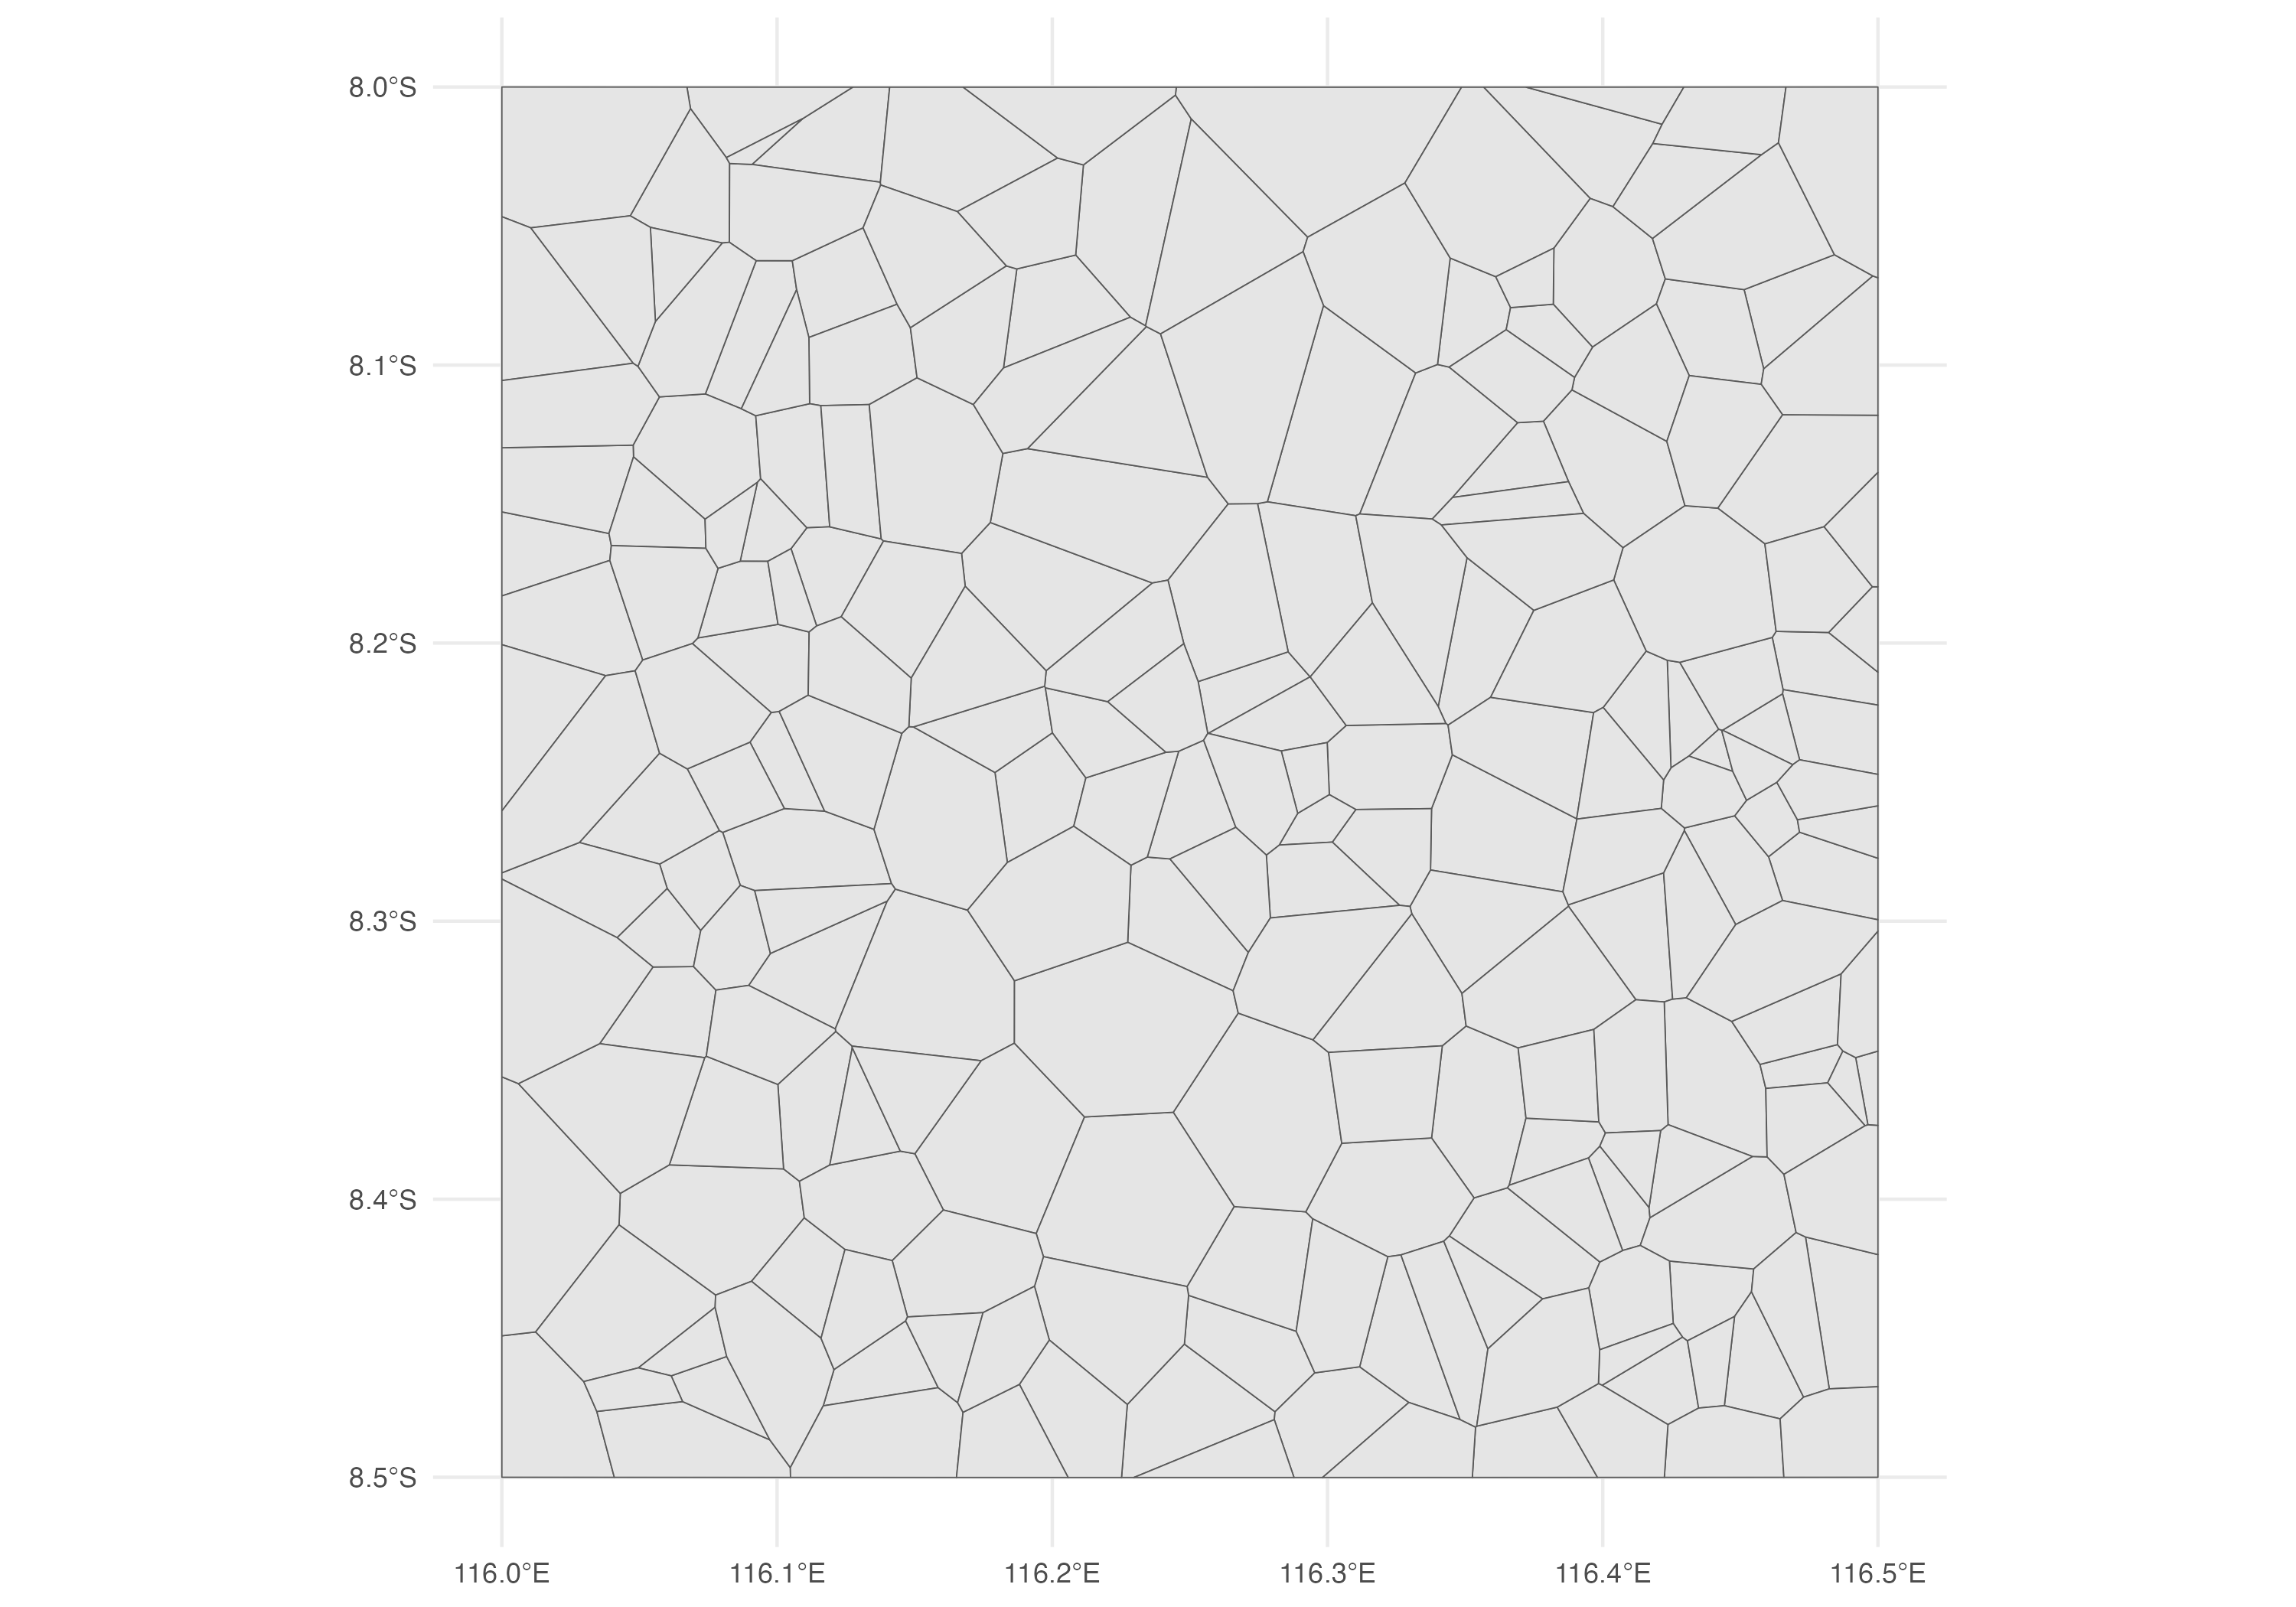
\includegraphics[width=1\textwidth,height=\textheight]{figures/artfcountry_plot.png}

}

\caption{\label{fig-artfreg}Artificial study region used for simulation
analysis, consisting of 216 non-overlapping polygonal areas. Each area
represents a distinct spatial unit for modelling and analysis, providing
a controlled environment to evaluate spatial models' performance}

\end{figure}%

\textsubscript{Source:
\href{https://indiraputeri-phd.github.io/CAR_simcomp/manuscript.qmd.html}{Article
Notebook}}

Another specific ingredient in spatial modelling is the existence of
\(W\) matrix, also known as the spatial weights matrix. It encodes the
spatial relationships between areas in a study region. The weight matrix
visually shows how different regions are connected to each other,
indicating their neighbourhood relationships (Morris et al. (2019)). To
demonstrate this concept, let's take a simple example of a map with 5
regions \((A, B, C, D, E)\), as visualised in
Figure~\ref{fig-neighsimple}.

\phantomsection\label{cell-fig-neighsimple}
\begin{figure}[H]

\centering{

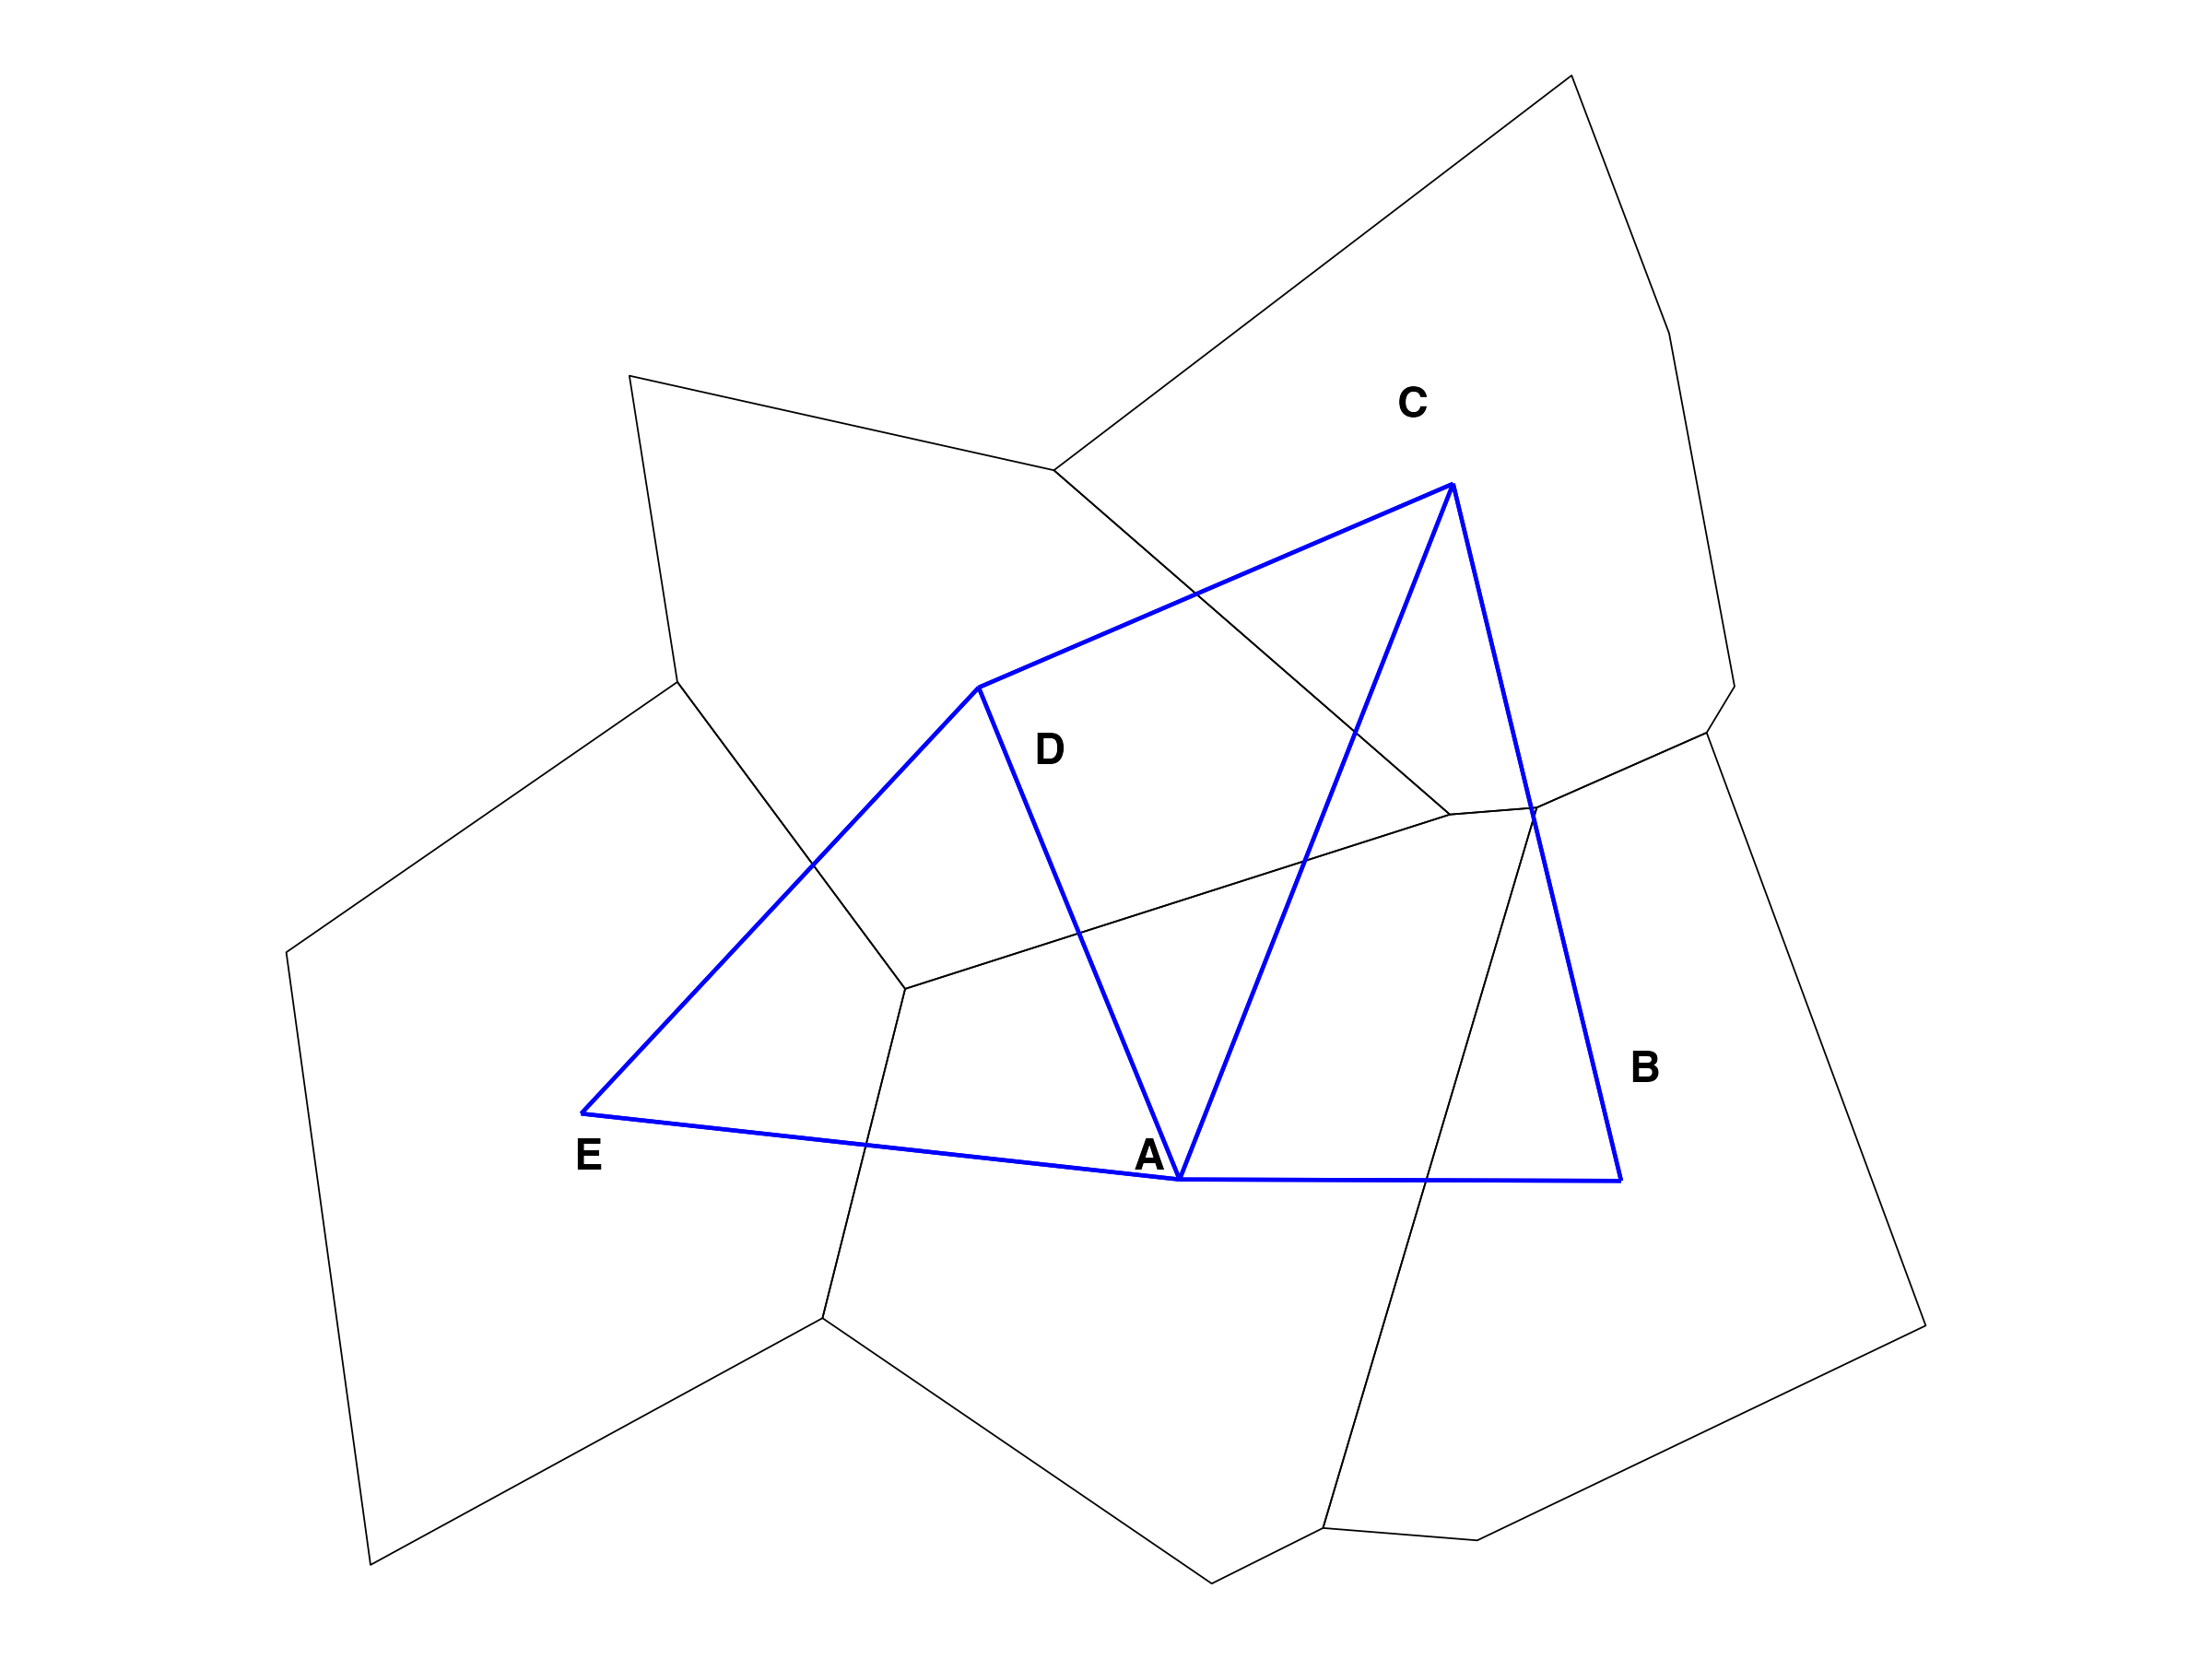
\includegraphics[width=0.5\textwidth,height=\textheight]{figures/sartf_plot.png}

}

\caption{\label{fig-neighsimple}Illustration of neighbourhood structure.
The figure depicts a simplified spatial configuration where each
numbered area represents a distinct spatial unit, demonstrating how
neighbouring relationships can be defined for spatial modelling
purposes.}

\end{figure}%

\textsubscript{Source:
\href{https://indiraputeri-phd.github.io/CAR_simcomp/manuscript.qmd.html}{Article
Notebook}}

From the Figure~\ref{fig-neighsimple} we can derive an adjacency matrix
which represents the neighborhood structure of five spatial units
labeled \(A\) to \(E\). Each entry 1 indicates a direct adjacency (areas
share a common border), while 0 denotes no direct connection. For
example, Area \(A\) is adjacent to all other areas (\(B\), \(C\), \(D\),
and \(E\)), whereas Area \(B\) is only adjacent to \(A\) and \(C\). This
neighbourhood configuration captures a clear spatial interaction pattern
among the areas, which forms the basis for constructing a spatial weight
matrix, commonly denoted as the \(\mathbf{W}\) matrix

\[
\begin{array}{cccccc}
    & A & B & C & D & E \\
A & 0 & 1 & 1 & 1 & 1\\ 
B & 1 & 0 & 1 & 0 & 0\\ 
C & 1 & 1 & 0 & 1 & 0\\
D & 1 & 0 & 1 & 0 & 1\\
E & 1 & 0 & 0 & 1 & 0\\
\end{array}
\]

Later on, in the modelling stage, we will also need to construct a
diagonal matrix \(\boldsymbol{D}\). It is an \(N \times N\) matrix where
each diagonal element \(d_{ii}\) denotes the number of neighbours of
region. while all non-diagonal elements are zero. This matrix is
essential in spatial econometric models because it captures the local
neighbourhood structure of each region. In the context of Geographically
Weighted Regression (GWR), Spatial Autoregressive (SAR), and Conditional
Autoregressive (CAR) models, \(\boldsymbol{D}\) plays a pivotal role in
defining spatial relationships and dependencies among different regions.

For instance, in SAR and CAR models, the diagonal matrix
\(\boldsymbol{D}\) aids in incorporating spatial lag and error
components by appropriately weighting the influence of neighbouring
regions (Wall (2004), Ver Hoef et al. (2018)). In GWR, this matrix
assists in locally calibrating the model by reflecting the density and
connectivity of regions (Brunsdon, Fotheringham, and Charlton (1996),
Stewart Fotheringham and Park (2018)). Here, \(\boldsymbol{D}\) is
represented as:

\[
\begin{array}{cccccc}
   & A & B & C & D & E \\
A & 4 & 0 & 0 & 0 & 0\\ 
B & 0 & 2 & 0 & 0 & 0\\ 
C & 0 & 0 & 3 & 0 & 0\\
D & 0 & 0 & 0 & 3 & 0\\
E & 0 & 0 & 0 & 0 & 2\\
\end{array}
\]

This matrix format indicates that region \(A\) has 4 neighbour, regions
\(C\) and \(D\) each have 3 neighbours, and region \(B\) and \(E\) has 2
neighbour.

\phantomsection\label{cell-fig-neighartfreg}
\begin{figure}[H]

\centering{

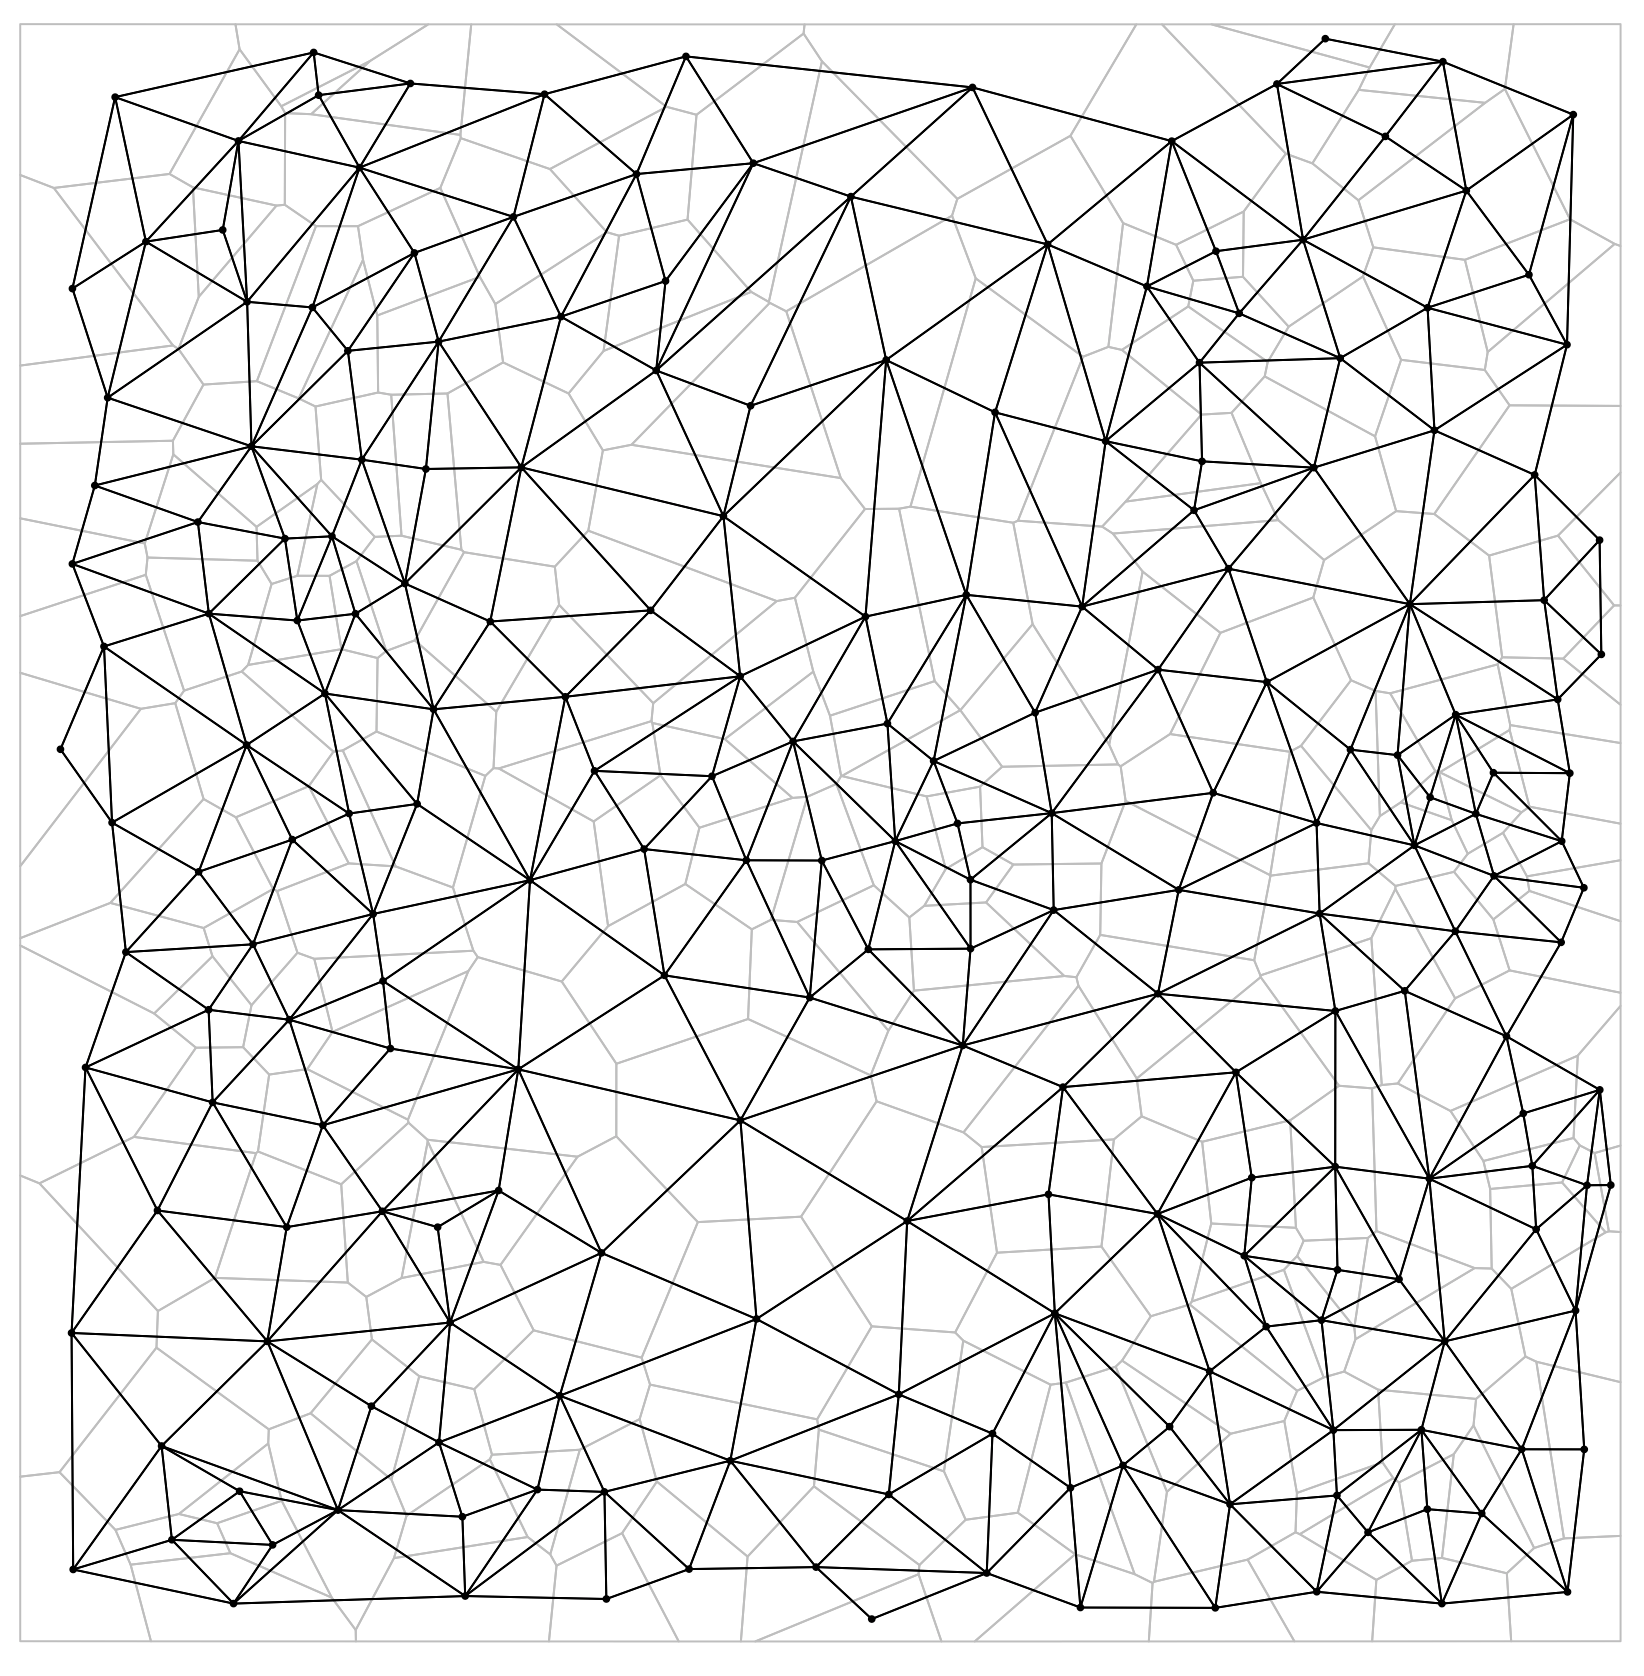
\includegraphics[width=0.7\textwidth,height=\textheight]{figures/nb_artfcountry.png}

}

\caption{\label{fig-neighartfreg}Neighbourhood structure of the
artificial region. This figure illustrates the spatial connectivity
between polygons in the artificial study region, where each line
represents a defined neighbour relationship based on spatial adjacency}

\end{figure}%

\textsubscript{Source:
\href{https://indiraputeri-phd.github.io/CAR_simcomp/manuscript.qmd.html}{Article
Notebook}}

In relation to our artificial study region,
Figure~\ref{fig-neighartfreg} illustrates the connections between areas,
represented by vertices or centroids for each area and nodes connecting
them to each other. This visualisation highlights the spatial adjacency
structure within the region.

\section{Spatial regression model}\label{spatial-regression-model}

When discussing spatial regression, it's crucial to comprehend the basic
notion of linear regression. In classical linear regression, the
relationship between the dependent variable \(y\) and the
\(x_1,x_2, \dots, x_p\) independent variables is expressed as

\begin{equation}\phantomsection\label{eq-basicreg}{
y = \beta_0 + \beta_1x_1 + \dots + \beta_p x_p + \varepsilon
}\end{equation}

This formulation assumes a global relationship between the variables,
where the coefficients \(\beta_1,\beta_2, \dots, \beta_p\) are constant
across the entire study area. In many spatial datasets, relationships
between variables may exhibit spatial variation. For example, in the
case of property pricing, a consistent rates of change assumption may
not hold true universally. For example, the house price increase for an
extra bedroom is often thought to be fixed across all locations.
However, local customs or knowledge may actually dictate these rates,
rather than a universal utility assigned to each commodity. For
instance, in neighbourhoods with families, where extra space is highly
valued, the perceived value of an additional bedroom may be greater
compared to areas with singles or elderly couples, for whom extra space
may not be as desirable.

\subsection{Geographically Weighted Regression
(GWR)}\label{geographically-weighted-regression-gwr}

Brunsdon, Fotheringham, and Charlton (1996) developed GWR which is one
such technique that extends classical linear regression by allowing
coefficients to vary spatially. It allows for the estimation of local
relationships between a response variable and predictor variables. It is
particularly useful for exploring spatial non-stationarity and
identifying spatially varying relationships across different locations.
The GWR model can be expressed as:

\begin{equation}\phantomsection\label{eq-gwr}{
y_i(s) = \beta_{0}(s) + \sum_{k=1}^p \beta_k(s)x_{ik}(s) + \varepsilon(s), \\ i = 1,\dots, n
}\end{equation}

Equation~\ref{eq-gwr} represents a spatial regression model where
\(\mathbf{y}(s)\) is the dependent variable at location \(s\). The term
\(\beta_{0}(s)\) is the spatially varying intercept, while
\(\sum_{k=1}^p \beta_k(s)\mathbf{x_k}(s)\) represents the spatially
varying coefficients for the independent variables \(\mathbf{x_k}(s)\).
\(\varepsilon(s)\) denotes the error term, capturing unexplained
variation at location \(s\)

Using a weighted least squares approach to calibrate regression models
allows different weights to be assigned to different observations,
influencing the estimated parameters. In ordinary least squares, the
goal is to minimize the sum of squared differences between predicted and
actual \(y\) values. Weighted least squares, however, apply a weighting
factor \(w\) to each squared difference, making some prediction
inaccuracies more significant. If \(w\) is a diagonal matrix of weights,
the estimated coefficients are given by Equation~\ref{eq-betagwr}:

\begin{equation}\phantomsection\label{eq-betagwr}{
\beta(s) = (\boldsymbol{x}^T \boldsymbol{W}(s) \boldsymbol{x})^{-1} \boldsymbol{x}^T \boldsymbol{W}(s) \boldsymbol{y}
}\end{equation}

This method allows GWR to address spatial heterogeneity by emphasizing
observations near the location of interest, thereby improving the
accuracy and relevance of local model estimates.

The estimation of GWR parameters involves fitting a separate regression
equation for each location in the study area. Various estimation
techniques can be employed, including ordinary least squares (OLS),
weighted least squares (WLS), and maximum likelihood estimation (MLE).
These techniques aim to optimize the model parameters to minimize the
differences between the observed and predicted values of the dependent
variable.

\subsection{Simultaneously Autoregressive (SAR)
Models}\label{simultaneously-autoregressive-sar-models}

While GWR focuses on capturing localised spatial heterogeneity by
allowing coefficients to vary across space, SAR take a different
approach by explicitly modelling spatial dependencies through a spatial
lag. The SAR model is a spatial econometric model used to analyse
spatial dependencies and relationships among observations in a
geographic space (Anselin and Griffith (1988)). It is widely employed in
various fields, such as regional economics, environmental studies, and
urban planning. SAR is a type of spatial autoregressive model involving
a simultaneous equation framework to capture spatial interactions.

The general form of SAR model can be expressed as follows

\begin{equation}\phantomsection\label{eq-sar}{
y(s) = \rho \sum_{s'} w(s,s') y(s') + \sum_{k=1}^p \beta_k x_k(s) + \varepsilon(s)
}\end{equation}

where \(\mathbf{Y}\) is the vector of observed values for the dependent
variable, \(W\) is the spatial weights matrix, \(\rho\) is the spatial
autoregressive coefficient, \(X\) is the matrix of observed values for
exogenous variables, \(\beta\) is the vector of coefficients, and
\(\boldsymbol{\varepsilon} \sim N(0,\sigma^2)\) is the vector of error
terms. Estimation of the SAR model parameters is typically done using
statistical techniques such as maximum likelihood estimation (MLE) or
generalised method of moments (GMM). The joint distribution of
\(\mathbf{Y}\) can be written as

\begin{equation}\phantomsection\label{eq-jointysar}{
\mathbf{Y} \sim \mathcal{N}\left( \left( I - \rho W \right)^{-1} X\beta, \, \sigma^2 \left( I - \rho W \right)^{-1} \left( I - \rho W^T \right)^{-1} \right)
}\end{equation}

Extensions of the SAR model include the Spatial Lag Model, the Spatial
Error Model, and the Spatial Durbin Model (Elhorst et al. (2014)), each
incorporating distinct assumptions regarding the spatial configuration
of the errors (Elhorst, Lacombe, and Piras (2012); Anselin (2013)).
These extensions provide flexibility to account for different types of
spatial dependencies and can be chosen based on the specific spatial
relationships and hypotheses under investigation.

The SAR model, with its various specifications, provides a flexible
framework to account for spatial dependencies and explore the spatial
dynamics of observed phenomena. Researchers often choose between these
models based on the nature of the spatial relationships in their data
and the specific hypotheses they aim to test. The SAR model is a
valuable tool for understanding spatial interdependence and making
informed policy and planning decisions in diverse spatial contexts

\subsection{Conditional Autoregressive (CAR)
Models}\label{conditional-autoregressive-car-models}

CAR models are a class of spatial statistical models used to analyze
spatially structured data. The general formulation of a CAR model can be
expressed as:

\begin{equation}\phantomsection\label{eq-car}{
y(s) = \sum_{k=1}^p \beta_k x_k(s) + \varepsilon(s) + \phi(s) 
}\end{equation}

Here, \(\boldsymbol{\varepsilon} \sim N(0, \nu^2)\) while
\(\boldsymbol{\phi}\) is a specific component in CAR model that has a
role as spatial effect. It is also common to mention
\(\boldsymbol{\phi}\) as a CAR priors. It is a type of Gaussian Markov
random field (Rue and Held (2005)), capture spatial autocorrelation by
ensuring that values at nearby locations are more similar than those
further apart (Lee (2013)). This can be expressed in a general term

\begin{equation}\phantomsection\label{eq-phidist}{
\boldsymbol{\phi}\sim N(0,\tau^2\boldsymbol{Q}^{-1}) 
}\end{equation}

where \(\boldsymbol{Q}\) is a precision matrix that may be singular
(intrinsic model). \(\boldsymbol{Q}\) controls the spatial
autocorrelation structure of the random effects, and is based on a
non-negative symmetric \(n \times n\) neighbourhood or weight matrix
\(\boldsymbol{W}\).

Together with the spatial weights matrix \(\boldsymbol{W}\), the prior
information are crucial components of CAR models. The choice of
\(\boldsymbol{W}\) determines the spatial structure of the model, while
the priors for the variance parameters and the spatial random effects
influence the model's ability to capture spatial dependencies. Commonly
used priors for the variance parameters include inverse-gamma
distributions, which provide flexibility and can be tuned to reflect
prior beliefs about the scale of variability in the data. The prevailing
approach typically involves a binary representation using geographical
adjacency, where \(w_{ki} = 1\) if areal units \((S_k,S_i)\) have a
mutual boundary (denoted \(k\sim i\), and is zero otherwise). This
specification forces \((\phi_k,\phi_i)\) relating to geographically
adjacent areas (that is \(w_{ki} = 1\)) to be correlated. On the other
hand, random effects associated with areas that are not adjacent are
independent of each other, provided we know the values of the other
random effects.

A CAR prior was introduced by Leroux, Lei, and Breslow (2000) and Stern
and Cressie (1999) to model diverse levels of spatial autocorrelation.
In this type of prior, a single collection of random effects is utilised
and its primary objective is to model spatial data, with a specific
focus on dealing with spatial relationships and auto-correlation between
data points. This model is especially proficient in the task of
smoothing data and detecting spatial patterns within data set. The
random effect \(\boldsymbol\phi_k\) structured as follow:

\begin{equation}\phantomsection\label{eq-phicar}{
\phi_k|\boldsymbol\phi_{-K}, \boldsymbol{W},\rho, \tau^2  \sim  N\left(\frac{\rho\sum_{i=1}^Kw_{ki}\phi_i}{A},\frac{\tau^2}{A}\right)
}\end{equation}

where \(A = \rho\sum_{i=1}^Kw_{ki}+1-\rho\). Note that when
\(\rho = 1\), the prior forms an intrinsic CAR prior (Besag, York, and
Mollié 1991), indicating full spatial dependency. Conversely, when
\(\rho = 0\), \(A = 1\) it means that there will be no \(W\) matrix role
in the model, and it will become a comman random effect. In other words,
the model reduces to a generalised linear model.

When handling \(i\) observations within each area \(k\),
Equation~\ref{eq-ycar} closely resembles Equation~\ref{eq-gwr} in the
GWR model, with the exception of the \(\phi\) component. It is usually
called multilevel CAR models

\begin{equation}\phantomsection\label{eq-ycar}{
y_i(s) = \sum_{k=1}^p \beta_k x_{ki}(s) + \varepsilon_i(s) + \phi(s)
}\end{equation}

The Bayesian approach to CAR models entails defining prior distributions
for all model parameters, such as the regression coefficients \(\beta\),
variance parameters \(\nu^2\) and \(\tau^2\), and spatial random effects
\(\phi_k\). Subsequently, Bayesian inference techniques like Markov
Chain Monte Carlo (MCMC) are employed to derive posterior distributions
of these parameters. This method facilitates the integration of prior
knowledge and offers a versatile framework for quantifying uncertainty.

In general, Table~\ref{tbl-summarymethod} below summarises the key
elements utilised in the GWR, SAR, and CAR models:

\begingroup\fontsize{9}{11}\selectfont

\begin{longtable}[t]{llll}

\caption{\label{tbl-summarymethod}Comparison of Model Elements Across
GWR, SAR, and CAR}

\tabularnewline

\toprule
Elements & $GWR$ & $SAR$ & $CAR$\\
\midrule
Number of Observations ($N$) & $\checkmark$ & $\checkmark$ & $\checkmark$\\
Covariate Matrix ($X$) & $\checkmark$ & $\checkmark$ & $\checkmark$\\
Spatial Weights Matrix ($W$) & $\times$ & $\checkmark$ & $\checkmark$\\
Spatial Coordinates (coords) & $\checkmark$ & $\checkmark$ & $\checkmark$\\
Covariate Coefficients ($\beta$) & $\checkmark$ & $\checkmark$ & $\checkmark$\\
\addlinespace
Error Term variance ($\sigma^2$) & $\checkmark$ & $\checkmark$ & $\checkmark$\\
Spatial Autocorrelation ($\rho$) & $\times$ & $\checkmark$ & $\checkmark$\\
Spatial Structure component ($\phi$) & $\times$ & $\times$ & $\checkmark$\\
Spatial structure variance ($\tau^2$) & $\times$ & $\times$ & $\checkmark$\\
Additional scale ($\nu^2$) & $\times$ & $\times$ & $\checkmark$\\
\addlinespace
Estimation method & MLE & MLE/GMM & MCMC\\
\bottomrule

\end{longtable}

\endgroup{}

\textsubscript{Source:
\href{https://indiraputeri-phd.github.io/CAR_simcomp/manuscript.qmd.html}{Article
Notebook}}

\section{Comparative Analysis of GLM, SAR, and
CAR}\label{comparative-analysis-of-glm-sar-and-car}

This section focuses on generating spatially autocorrelated property
price data, exploring two distinct data generation frameworks: one using
a CAR specification and another without spatial autocorrelation
(non-CAR). The analysis is conducted within an artificially constructed
study area using key property covariates: land size, building size,
number of bedrooms, and number of bathrooms. The generated datasets are
then employed to examine spatial dependencies in property prices and are
analysed using a suite of models including GLM, SAR, and CAR.

\subsection{The experiment design}\label{the-experiment-design}

The experiment begins by creating a dataset based on the defined study
region. The idea is to generate covariates that hypothetically can
explain price of a property. It basically consist of property structural
characteristics such as land size, building size, number of bedrooms,
and number of bathrooms. To represent real-world data, each polygon
contains multiple observations.

To generate the covariates, the first step involves creating area-level
data with a specific spatial pattern, referred to as the housing density
for the study region. The spatial pattern implies that certain areas or
polygons will have a higher housing density than others. In this case,
the central horizontal region of the study area is set to has a higher
housing density, mirroring the housing distribution found on the island
of Lombok. Although this density will not be directly utilized in the
model simulation, it serves as a critical foundation for determining the
spatial distribution of observation points across each polygon. In areas
with higher density, a greater number of observation points are
generated, which aligns with the notion that densely populated regions
typically have more residential developments, thereby increasing the
number of properties available for sale. Across the 216 polygons, a
total of 4,314 observation points were generated. The number of
observations per polygon varies from 5 to 56 points, reflecting the
density in each area. Figure~\ref{fig-pointsonmap} illustrate how each
polygon has multiple observations and they are distributed according to
a specific pattern.

\phantomsection\label{cell-fig-pointsonmap}
\begin{figure}[H]

\centering{

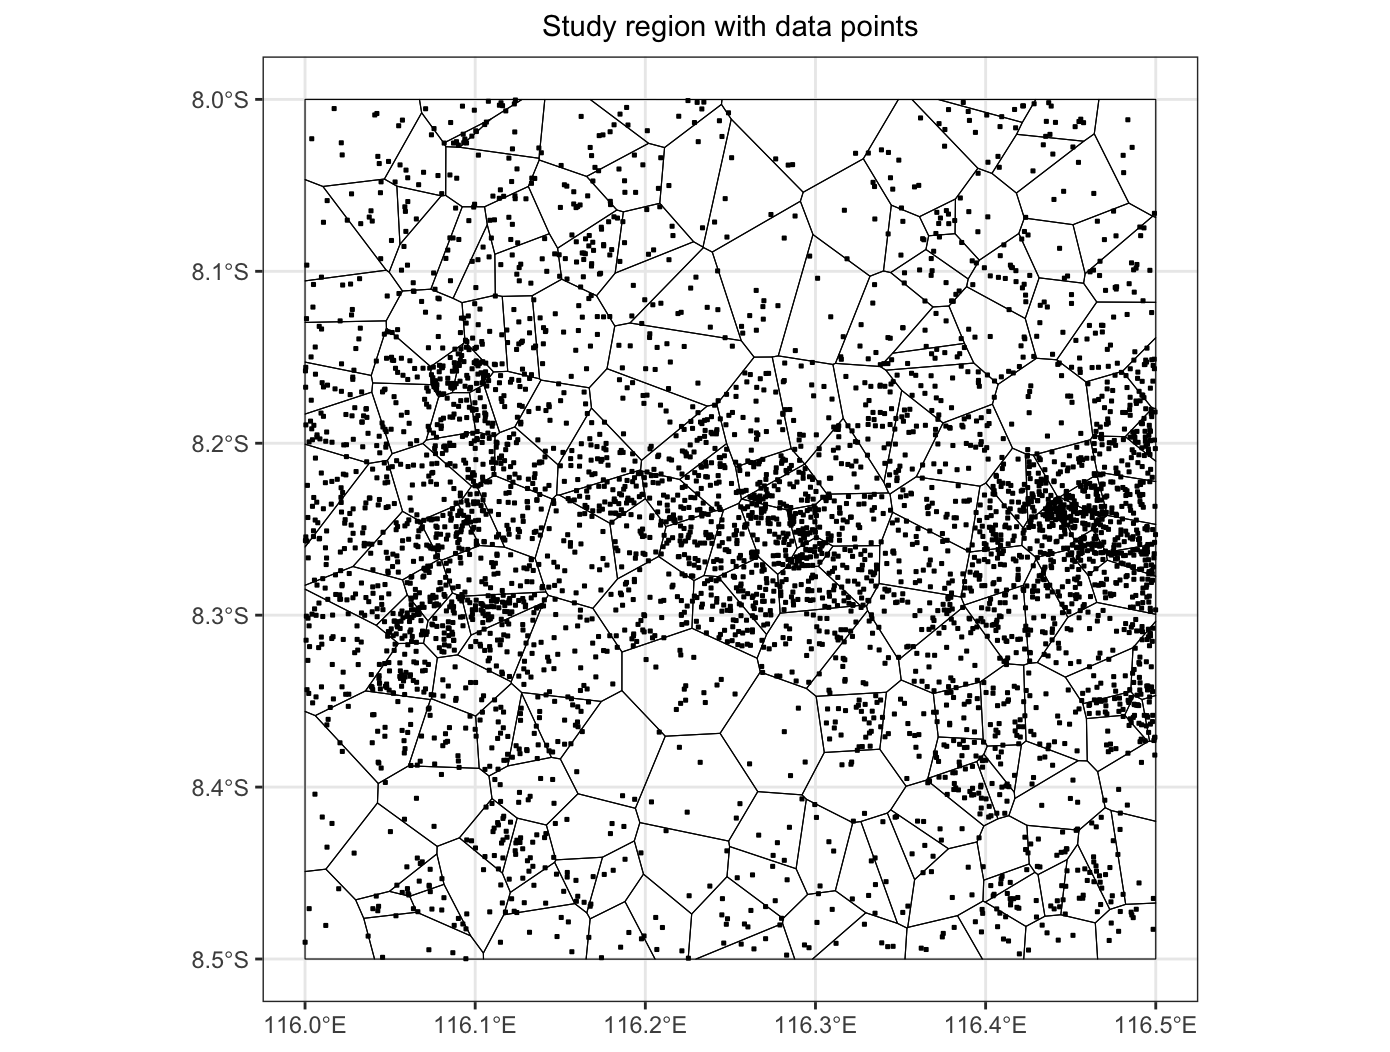
\includegraphics[width=0.8\textwidth,height=\textheight]{figures/density_points_plot.png}

}

\caption{\label{fig-pointsonmap}Artificial study region with observation
points. The points represent data locations within each polygon,
simulating real-world spatial observations for the purpose of model
analysis and validation.}

\end{figure}%

\textsubscript{Source:
\href{https://indiraputeri-phd.github.io/CAR_simcomp/manuscript.qmd.html}{Article
Notebook}}

Following this, covariates were generated using \texttt{mvrnorm()} for
each observation point, creating a dataset for further analysis.
Table~\ref{tbl-covrstr} provides a brief slice of the covariates'
structure.

\begingroup\fontsize{9}{11}\selectfont

\begin{longtable}[t]{rrrrr}

\caption{\label{tbl-covrstr}Slice of generated dataset as covariates for
simulations}

\tabularnewline

\toprule
ID & land\_size & building\_size & \#bedrooms & \#bathrooms\\
\midrule
1 & 270.48 & 108.55 & 4 & 2\\
1 & 295.99 & 100.13 & 4 & 2\\
2 & 319.52 & 126.31 & 3 & 1\\
2 & 325.01 & 120.84 & 4 & 3\\
2 & 294.15 & 144.05 & 4 & 3\\
\addlinespace
3 & 222.18 & 81.40 & 3 & 2\\
4 & 414.23 & 150.15 & 2 & 2\\
4 & 278.75 & 101.41 & 2 & 1\\
\bottomrule

\end{longtable}

\endgroup{}

\textsubscript{Source:
\href{https://indiraputeri-phd.github.io/CAR_simcomp/manuscript.qmd.html}{Article
Notebook}}

By employing artificially generated covariates and an artificially
constructed study region, we developed three distinct property price
datasets, each based on a different spatial model: CAR, a combination of
CAR and SAR, and GWR. The true parameter values for this purpose are
\(\boldsymbol{\beta} = \begin{bmatrix} 1 & 0.9 & 0.7 & 0.5 & 0.3 \end{bmatrix}\),
\(\nu^2 = 0.2\), \(\tau^2 = 0.6\) and \(\rho = 0.6\). Whereas beta
values for GWR dataset is generated using a beta function, which is a
function of coordinate points. The matrix \(\mathbf{W}\) was derived
from the neighbourhood structure of an artificial study region using the
functions \texttt{poly2nb()} and \texttt{nb2mat()}. Data generation for
\(SAR + CAR\) employs a slightly different strategy. In addition to
being generated per area simultaneously using the joint distribution of
\(\mathbf{Y}\) as in Equation~\ref{eq-jointysar}, information about the
spatial effect \(\boldsymbol{\phi}\) is also added at the end of the
process. Therefore, we refer to it as \(SAR + CAR\) data.

Each data generation resulting two types of datasets: area-level and
point-level. These datasets were then modelled using six linear
regression approaches, comprising both classical and spatial regression
models: GLM, SAR, and CAR for area-level data, and GWR, GLMM, and
multilevel CAR for point-level data. Simulations were conducted
\(sim = 1000\) times. From each simulation, coefficients, parameters,
and fitted values were extracted, allowing for the computation of bias
and RMSE values for robustness and prediction power analysis.

\subsection{Robustness and power prediction
analysis}\label{robustness-and-power-prediction-analysis}

The bias values are summarised in Table~\ref{tbl-bias1} and
Table~\ref{tbl-bias2}. It shows that the models exhibit varying levels
of accuracy across the different parameters and datasets.
Figure~\ref{fig-biasplot} presents the bias estimates of regression
coefficients for different modelling approaches, separated by data type:
(a) area-level data and (b) point-level data. Each panel corresponds to
a data-generating mechanism (CAR, GWR, or SAR+CAR), and bias values are
shown with 95\% confidence intervals.

\begin{figure}

\begin{minipage}{0.50\linewidth}

\centering{

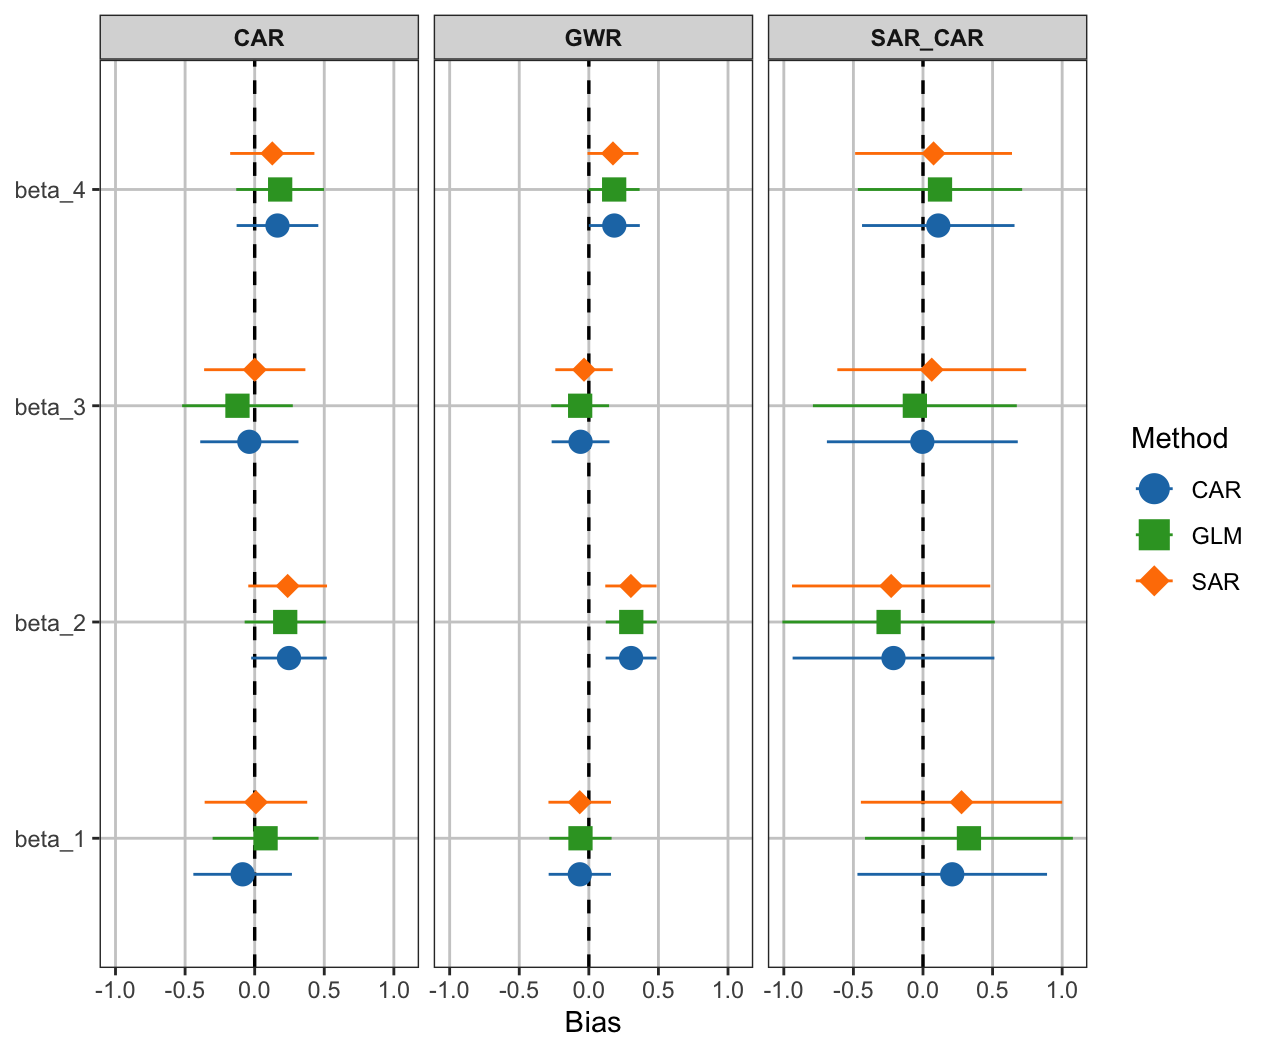
\includegraphics{figures/bias1_plot.png}

}

\subcaption{\label{fig-biasplot1}Bias values by method and dataset type
for area-level data}

\end{minipage}%
%
\begin{minipage}{0.50\linewidth}

\centering{

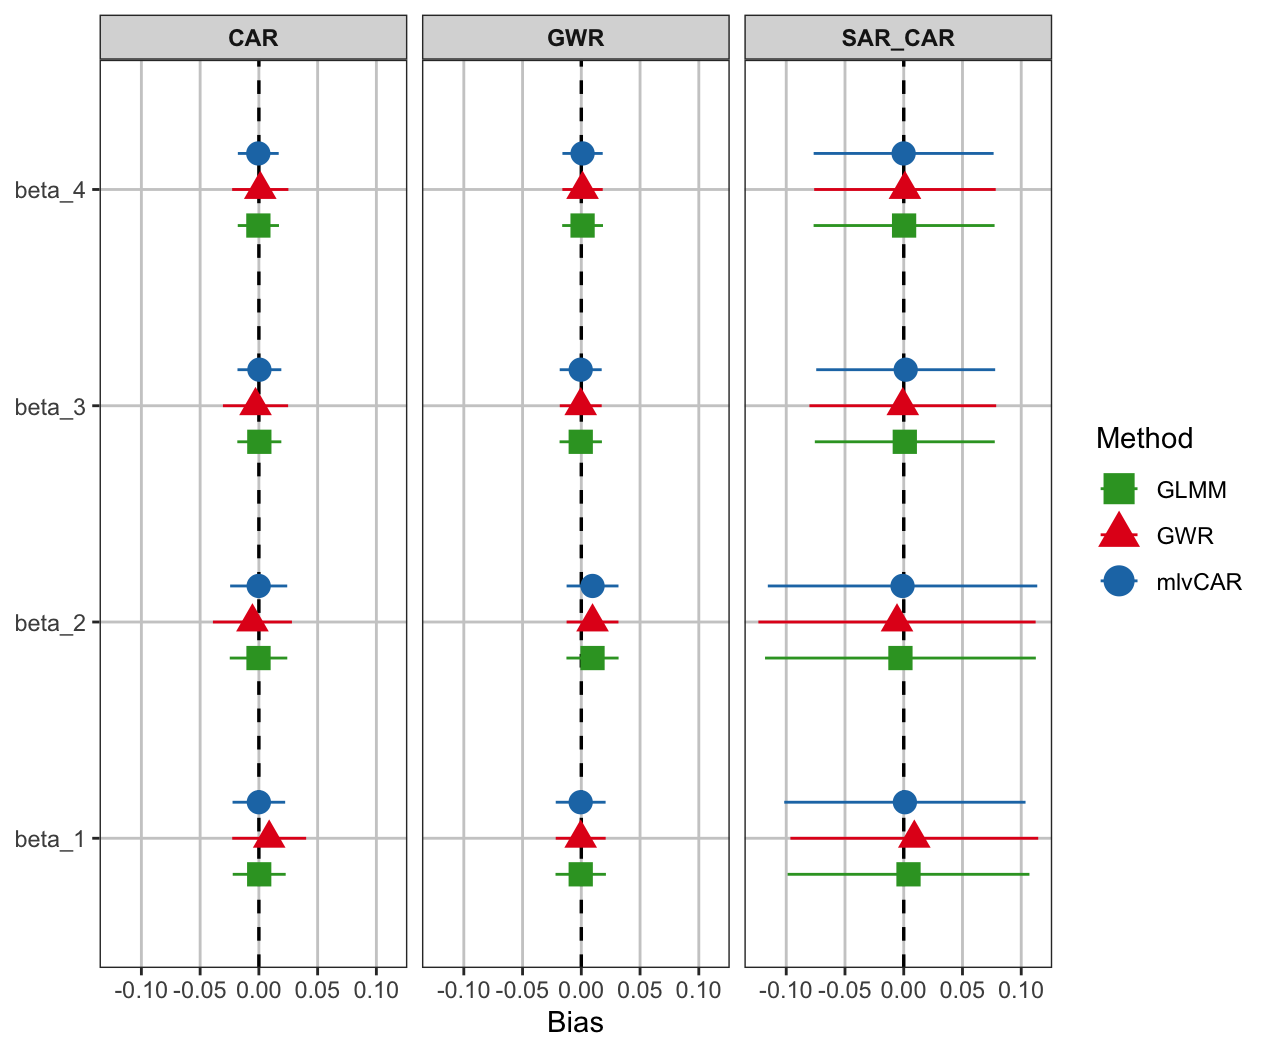
\includegraphics{figures/bias2_plot.png}

}

\subcaption{\label{fig-biasplot2}Bias values by method and dataset type
for point-level data}

\end{minipage}%

\caption{\label{fig-biasplot}Bias estimates comparison of six different
methods across datasets generated under CAR, GWR, and SAR+CAR
frameworks. Each method's performance is visualised for \(\beta_1\),
\(\beta_2\), \(\beta_3\), and \(\beta_4\), highlighting variations in
bias and the effectiveness of each model in addressing spatial
dependencies.}

\end{figure}%

\textsubscript{Source:
\href{https://indiraputeri-phd.github.io/CAR_simcomp/manuscript.qmd.html}{Article
Notebook}}

For area-level data (Figure~\ref{fig-biasplot1}), CAR model consistently
produces the lowest bias across all coefficients and data-generating
scenarios. This confirms its ability to recover true parameter values
under spatial dependency, even when data is aggregated. The SAR model
displays higher variability and often substantial bias, especially in
CAR-generated datasets, suggesting model misspecification when the true
structure is localised (as in CAR). GLM, which ignores spatial effects,
performs reasonably in some settings but often underperforms compared to
CAR.

In the point-level setting (Figure~\ref{fig-biasplot2}), the mlvCAR
model shows superior performance, achieving minimal bias across all
coefficients and data-generating mechanisms. This reflects its strength
in modeling spatial dependencies while accounting for multilevel data
structure (i.e., multiple observations within areas). GLMM performs
moderately well but tends to show slightly higher bias than mlvCAR. In
contrast, GWR, despite being designed for point-level spatial variation,
yields higher bias, especially under SAR+CAR structures. This suggests
GWR's limitation when spatial heterogeneity is not smooth or when model
assumptions are violated.

\begingroup\fontsize{9}{11}\selectfont

\begin{longtable}[t]{lrrrrrr}

\caption{\label{tbl-rmse}RMSE values across different datasets}

\tabularnewline

\toprule
\multicolumn{1}{c}{ } & \multicolumn{3}{c}{Area-level data} & \multicolumn{3}{c}{Point-level data} \\
\cmidrule(l{3pt}r{3pt}){2-4} \cmidrule(l{3pt}r{3pt}){5-7}
Dataset & $GLM$ & $SAR$ & $CAR$ & $GLMM$ & $GWR$ & $mlvCAR$\\
\midrule
\endfirsthead
\multicolumn{7}{@{}l}{\textit{(continued)}}\\
\toprule
\multicolumn{1}{c}{ } & \multicolumn{3}{c}{Area-level data} & \multicolumn{3}{c}{Point-level data} \\
\cmidrule(l{3pt}r{3pt}){2-4} \cmidrule(l{3pt}r{3pt}){5-7}
Dataset & $GLM$ & $SAR$ & $CAR$ & $GLMM$ & $GWR$ & $mlvCAR$\\
\midrule
\endhead

\endfoot
\bottomrule
\endlastfoot
$CAR$ & 4.09 & 3.85 & 1.81 & 14.04 & 21.13 & 9.94\\
$SAR + CAR$ & 11.88 & 11.68 & 3.88 & 47.67 & 48.87 & 38.97\\
$GWR$ & 2.43 & 2.42 & 2.28 & 18.31 & 18.33 & 14.87\\*

\end{longtable}

\endgroup{}

\textsubscript{Source:
\href{https://indiraputeri-phd.github.io/CAR_simcomp/manuscript.qmd.html}{Article
Notebook}}

Moreover, Table~\ref{tbl-rmse} provide insights into model accuracy at
different spatial levels. For area-level data, the models GLM, SAR, and
CAR are compared, with the CAR model consistently achieving the lowest
RMSE. This suggests that CAR is more effective at capturing spatial
dependencies at the area level. For point-level data, the models GLMM,
GWR, and mlvCAR are evaluated, with mlvCAR showing the lowest RMSE
across all datasets. This indicates that mlvCAR is particularly
well-suited for handling detailed spatial variations at the point level.
Overall, these results highlight the strengths of CAR and mlvCAR in
reducing error within their respective spatial contexts, underscoring
their potential utility in spatial modeling applications.

\section{Applications in Lombok house prices
dataset}\label{applications-in-lombok-house-prices-dataset}

In this section, we apply the simulated models to property price data on
Lombok Island, Indonesia. Lombok is located in the eastern part of
Indonesia, specifically between latitudes -8.9° and -8.1°, and
longitudes 115.9° and 116.6°.

\phantomsection\label{cell-fig-lombokmap}
\begin{figure}[H]

\centering{

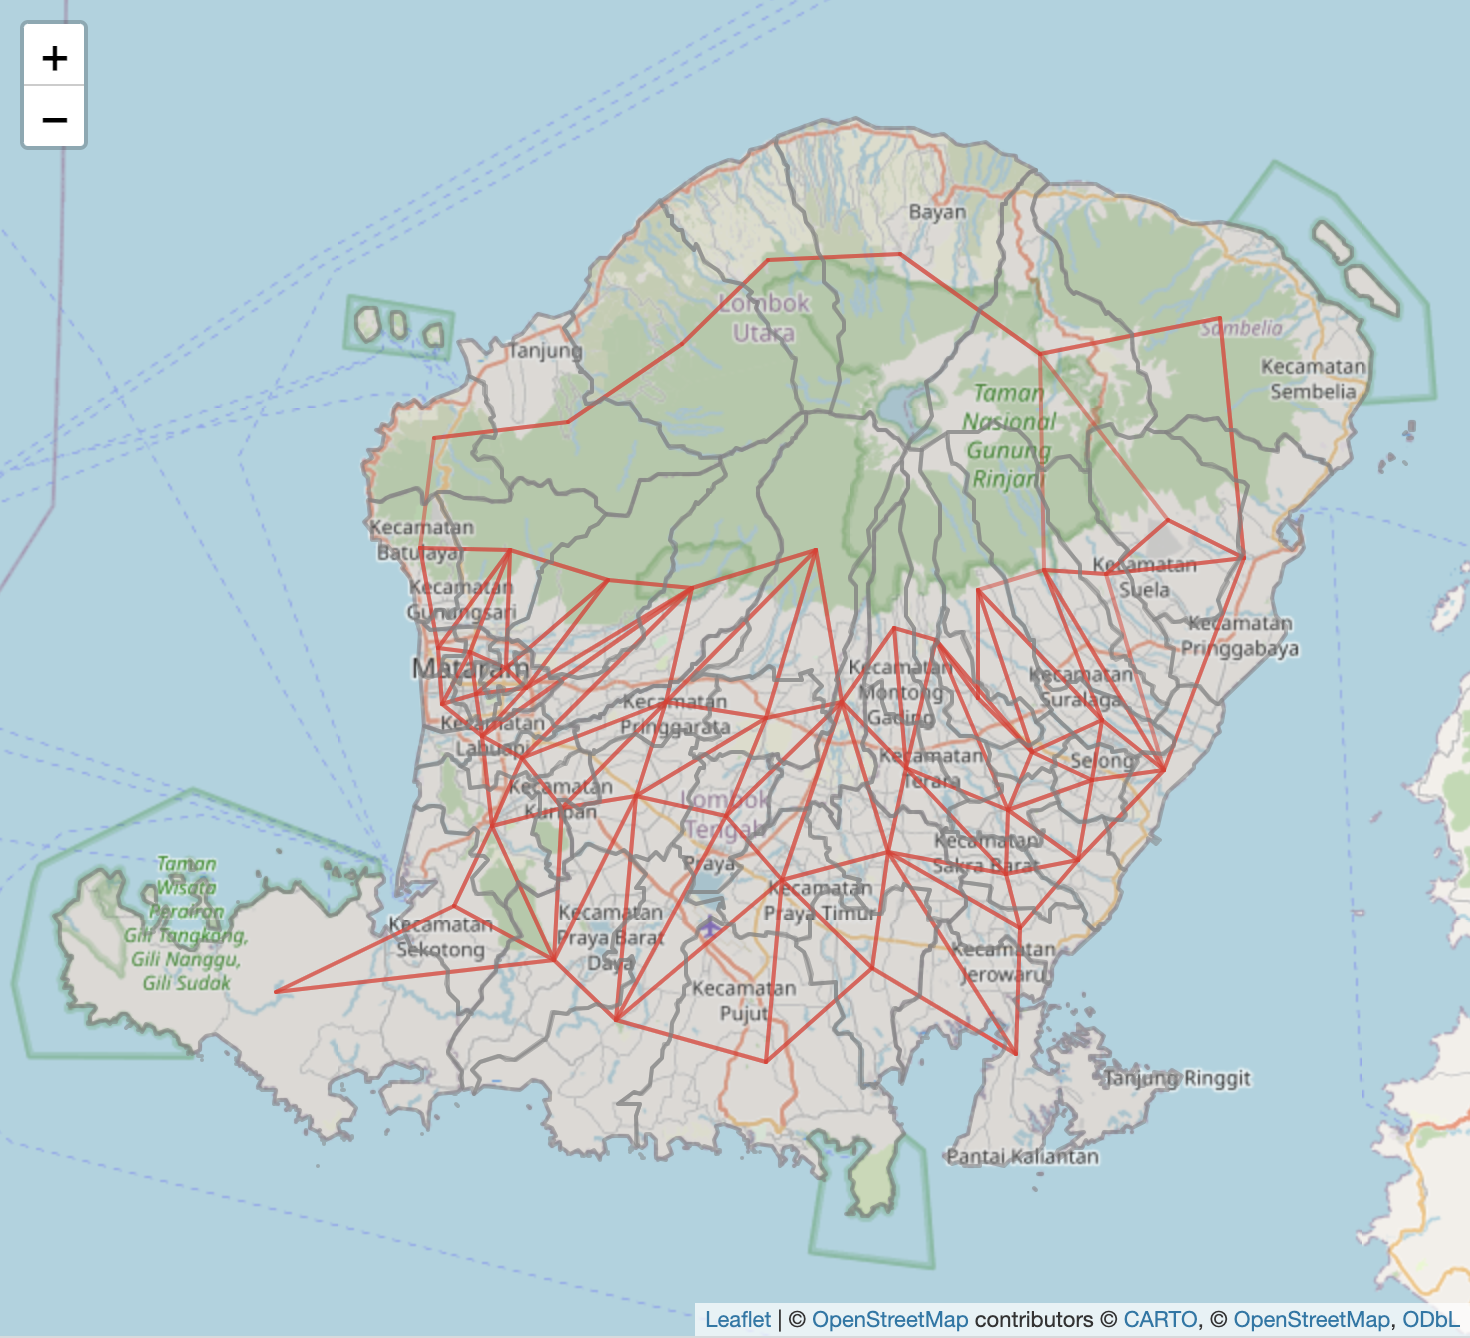
\includegraphics[width=0.75\textwidth,height=\textheight]{figures/nb_lop2.png}

}

\caption{\label{fig-lombokmap}Lombok neighbour structure at the
sub-district (Kecamatan) level. This figure illustrates the spatial
neighbour structure of sub-districts on Lombok Island. The red lines
represent the connections between neighbouring sub-districts based on
adjacency relationships, overlaid on a base map.}

\end{figure}%

\textsubscript{Source:
\href{https://indiraputeri-phd.github.io/CAR_simcomp/manuscript.qmd.html}{Article
Notebook}}

Lombok includes five districts (kota/kabupaten), 53 sub-districts
(kecamatan), and 608 villages (desa/kelurahan), which represent three
successive levels of administrative division. In this study, the
sub-district level is used as the spatial unit of analysis, as
illustrated in Figure~\ref{fig-lombokmap}. The key variables of interest
include property price, land size, built-up area, number of bedrooms,
and number of bathrooms.

\subsection{Data Collection}\label{data-collection}

Data were collected from multiple online sources. Property prices and
their associated characteristics were harvested using web-scraping
techniques from three leading Indonesian property trading platforms,
https://www.lamudi.co.id/, https://www.99.co/, and
https://www.rumah123.com/. The accuracy of the web-scraped data was
ensured by cross-referencing it with official datasets, performing
checks for missing or inconsistent entries, and validating key variables
through sample comparisons with manually collected data. From this
process, the initial dataset comprised 1,188 entries, with 9 variables,
including village, prices, land-size, built-up area, number of bedrooms,
number of bathrooms, floors, property type/category, and furnishing
status.

Further, we conducted several preprocessing steps. First, we filtered
the dataset by removing irrelevant variables, including floors,
furnishing status, and category. It was then subsequently filtered to
retain only properties with plausible characteristics: land area between
90 and 800 square meters, built-up size between 70 and 600 square
meters, a maximum of 6 bedrooms, and a maximum 5 bathrooms. These
thresholds were applied to ensure the data reflect realistic and
context-appropriate housing characteristics in Lombok, based on common
residential patterns and local housing norms. This step was essential to
enhance the validity of the analysis by excluding outliers or
potentially erroneous entries. Following this procedure, the dataset was
refined to comprise a total of 576 observations. A summary of the key
variables is presented in Table~\ref{tbl-datasumm}.

\begingroup\fontsize{9}{11}\selectfont

\begin{longtable}[t]{lrrrrrrrr}

\caption{\label{tbl-datasumm}Summary statistics of variables in the
property price dataset}

\tabularnewline

\toprule
Variable & Mean & Median & $Q_1$ & $Q_3$ & Min & Max & SD & NA\\
\midrule
Prices (million IDR) & 1983.00 & 1400 & 800.0 & 2500.0 & 170 & 22500 & 2056.81 & 26\\
Land-size (sqm) & 299.60 & 255 & 147.2 & 407.2 & 90 & 800 & 179.39 & 24\\
Built-up area (sqm) & 184.80 & 150 & 100.0 & 210.0 & 70 & 600 & 109.20 & 24\\
No. of bedroom & 3.24 & 3 & 2.0 & 4.0 & 1 & 6 & 1.19 & 24\\
No. of bathroom & 2.55 & 2 & 2.0 & 3.0 & 1 & 5 & 1.05 & 24\\
\bottomrule

\end{longtable}

\endgroup{}

\textsubscript{Source:
\href{https://indiraputeri-phd.github.io/CAR_simcomp/manuscript.qmd.html}{Article
Notebook}}

Next, we merged the cleaned dataset with spatial administrative data by
matching sub-district and district names. This process resulted in a
dataset containing 598 entries. Compared to the previous dataset, which
consisted of 576 observations, this indicates that 22 sub-districts did
not have any property data available---meaning that property sales in
those areas were not recorded on the online property listing platform
used as the data source.

To address missing values, we employed the \texttt{mice} package (Van
Buuren and Groothuis-Oudshoorn (2011)) to perform multiple imputation
with parameters set to \(maxit = 10\), \(m = 10\), and a fixed random
seed to ensure reproducibility. The imputed values were then
reintegrated into the main dataset, replacing the original missing
entries. This process resulted in a final dataset that was complete and
ready for subsequent analysis using the selected spatial models.

In addition to the point-level dataset, which contains individual
property listings, the imputed dataset was also aggregated to the
sub-district level by calculating the mean values of key variables. This
aggregation produced an area-level dataset, allowing the analysis to be
conducted at both the individual and administrative levels. These two
levels of data granularity provide complementary perspectives for
evaluating the performance of spatial models in capturing local property
market dynamics.

\subsection{Model Implementation \&
Analysis}\label{model-implementation-analysis}

The cleaned and completed Lombok dataset was then model. The tables
below present the results of the data fitting, offering a comparative
view of each model's effectiveness and accuracy in capturing the
dataset's characteristics.

\begin{equation}\phantomsection\label{eq-lopreg}{
prices \sim land_{std} + building_{std} + beds_{std} + baths_{std}
}\end{equation}

Standardization of the predictors ensures that the resulting
coefficients are on a comparable scale, facilitating meaningful
interpretation and comparison across different modeling approaches. The
results presented in Table~\ref{tbl-modelcomp} provide a comprehensive
evaluation of each model's performance in capturing both the structural
and spatial characteristics of the property market in Lombok.

We conducted model fitting on the area-level data, with detailed results
provided in the Appendix (Table~\ref{tbl-modelcomp1}). However, this
method does not provide optimal parameter estimates because data
aggregation can reduce variability and obscure spatial details essential
for capturing local effects. To address this, we used point-level data
to apply three different models: GLMM, GWR, and multilevel CAR.

\begin{table}

\caption{\label{tbl-modelcomp}Point-level Model Comparison}

\centering{

\centering\begingroup\fontsize{9}{11}\selectfont

\begin{tabular}[t]{llll}
\toprule
 & GLMM & GWR & mlvCAR\\
\midrule
\addlinespace[0.3em]
\multicolumn{4}{l}{\textbf{Coefficients}}\\
\hspace{1em}Intercept & 7.09 [6.93, 7.24]* & 7.25 [7.25, 7.26]* & 7.08 [6.99, 7.17]*\\
\hspace{1em}Land-size & 0.26 [0.21, 0.32]* & 0.31 [0.30, 0.32]* & 0.26 [0.21, 0.32]*\\
\hspace{1em}Built-up area & 0.16 [0.10, 0.22]* & 0.19 [0.19, 0.20]* & 0.16 [0.10, 0.21]*\\
\hspace{1em}No. of bedroom & -0.03 [-0.09, 0.01] & -0.15 [-0.17, -0.15]* & -0.03 [-0.09, 0.02]\\
\hspace{1em}No. of bathroom & 0.19 [0.13, 0.25]* & 0.24 [0.23, 0.26]* & 0.19 [0.13, 0.25]*\\
\addlinespace[0.3em]
\multicolumn{4}{l}{\textbf{Spatial parameter}}\\
\hspace{1em}$\rho$ & - & - & 0.48 [0.07, 0.90]*\\
\addlinespace[0.3em]
\multicolumn{4}{l}{\textbf{Variances}}\\
\hspace{1em}$\nu^2$ & 0.22 [0.19, 0.25]* & 0.33 [0.29, 0.37]* & 0.22 [0.20, 0.25]*\\
\hspace{1em}$\tau^2$ & 0.20 [0.11, 0.34]* & - & 0.31 [0.14, 0.58]*\\
\addlinespace[0.3em]
\multicolumn{4}{l}{\textbf{Model fit criterion}}\\
\hspace{1em}AIC & 803.38 & -645.104 & 786.95\\
\hspace{1em}DIC & - & - & 850.39\\
\hspace{1em}WAIC & 838.3 & - & 851.14\\
\hspace{1em}LMPL & -421.31 & - & -427.21\\
\hspace{1em}Log-likelihood & -400.69 & -520.97 & -385.47\\
\bottomrule
\end{tabular}
\endgroup{}

}

\end{table}%

\textsubscript{Source:
\href{https://indiraputeri-phd.github.io/CAR_simcomp/manuscript.qmd.html}{Article
Notebook}}

Here, Table~\ref{tbl-modelcomp} compares parameter estimates and fit
criteria for three models: GLMM, GWR, and multilevel CAR. Significant
coefficients are marked with an asterisk (*). Key determinants like
land-size and built-up area have positive, significant effects across
models, while the number of bedrooms shows only minor, varying effects,
indicating model-specific differences in capturing this variable's
influence. Only the multilevel CAR model includes the spatial parameter
\(\rho\), with a significant estimate of 0.48, showing the model's
ability to account for spatial dependence. Variance components \(\nu^2\)
(residual) and \(\tau^2\) (spatial) are also detailed, with both
variance terms significant. Fit criteria (AIC, WAIC, and Log-likelihood)
suggest mlvCAR and GWR may better capture local spatial variation, with
mlvCAR balancing spatial structure and precision.

\begin{figure}

\begin{minipage}{0.50\linewidth}

\centering{

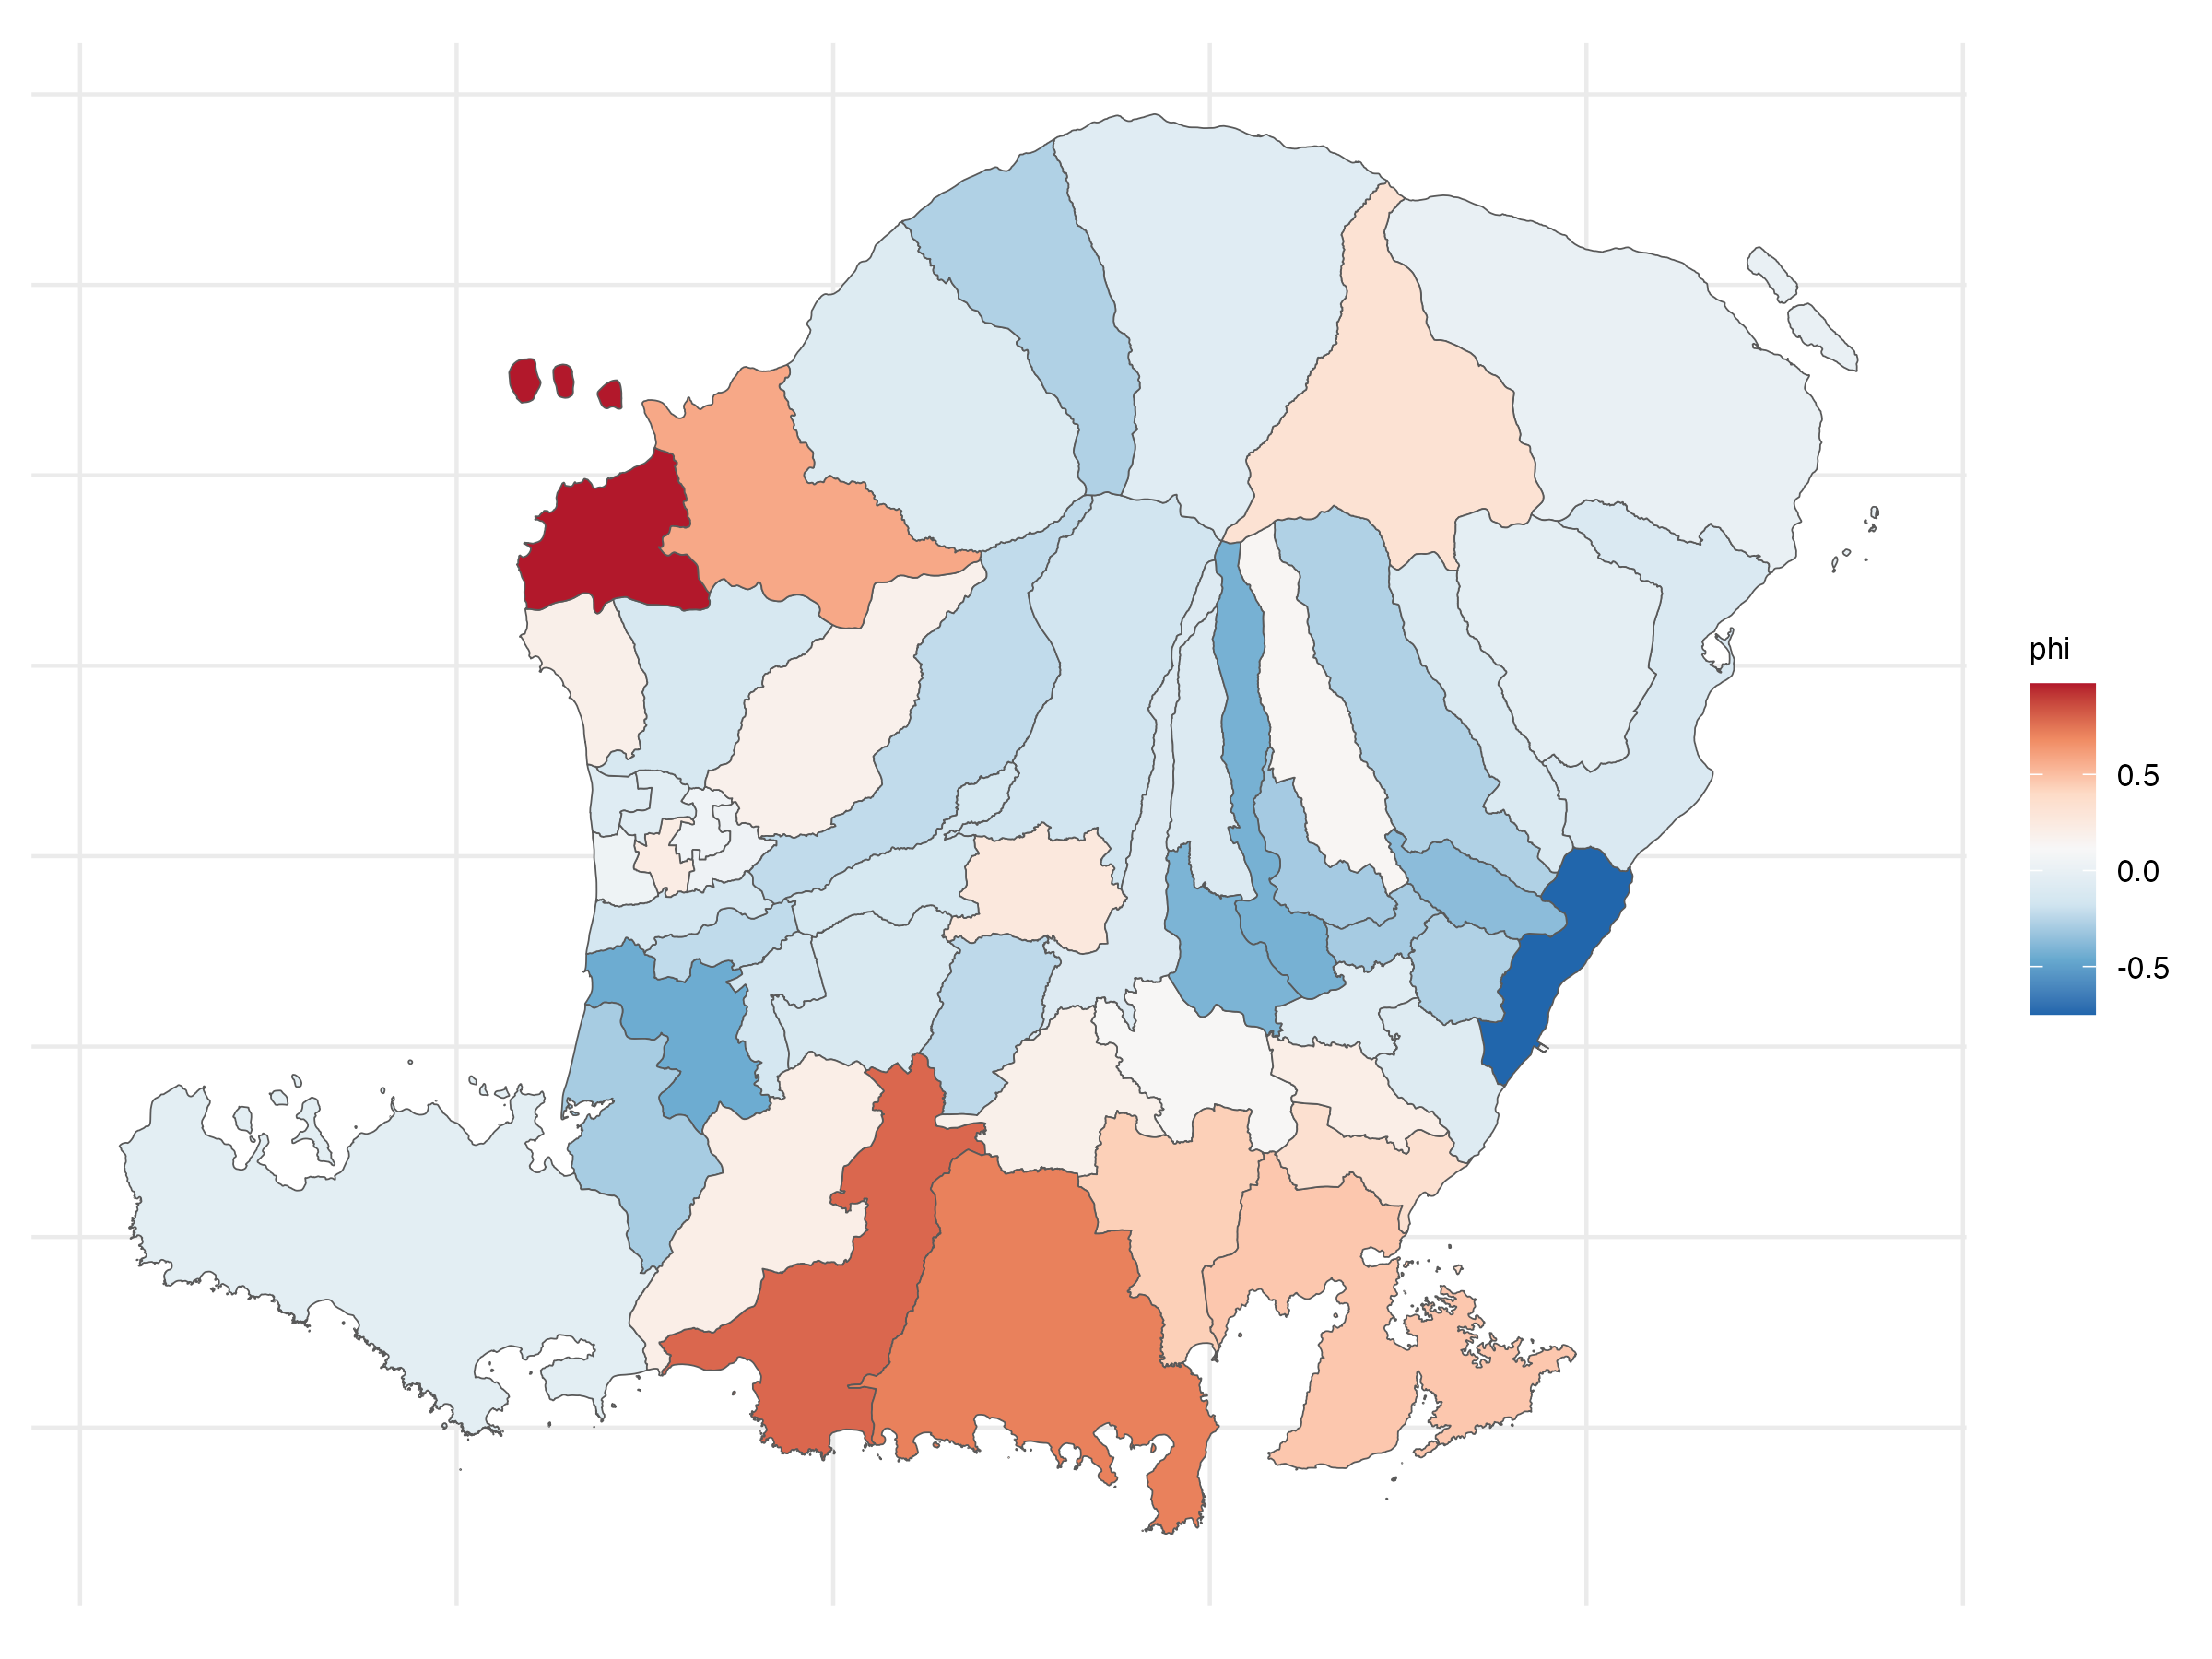
\includegraphics{figures/phi_map.png}

}

\subcaption{\label{fig-pricenphi1}phi values}

\end{minipage}%
%
\begin{minipage}{0.50\linewidth}

\centering{

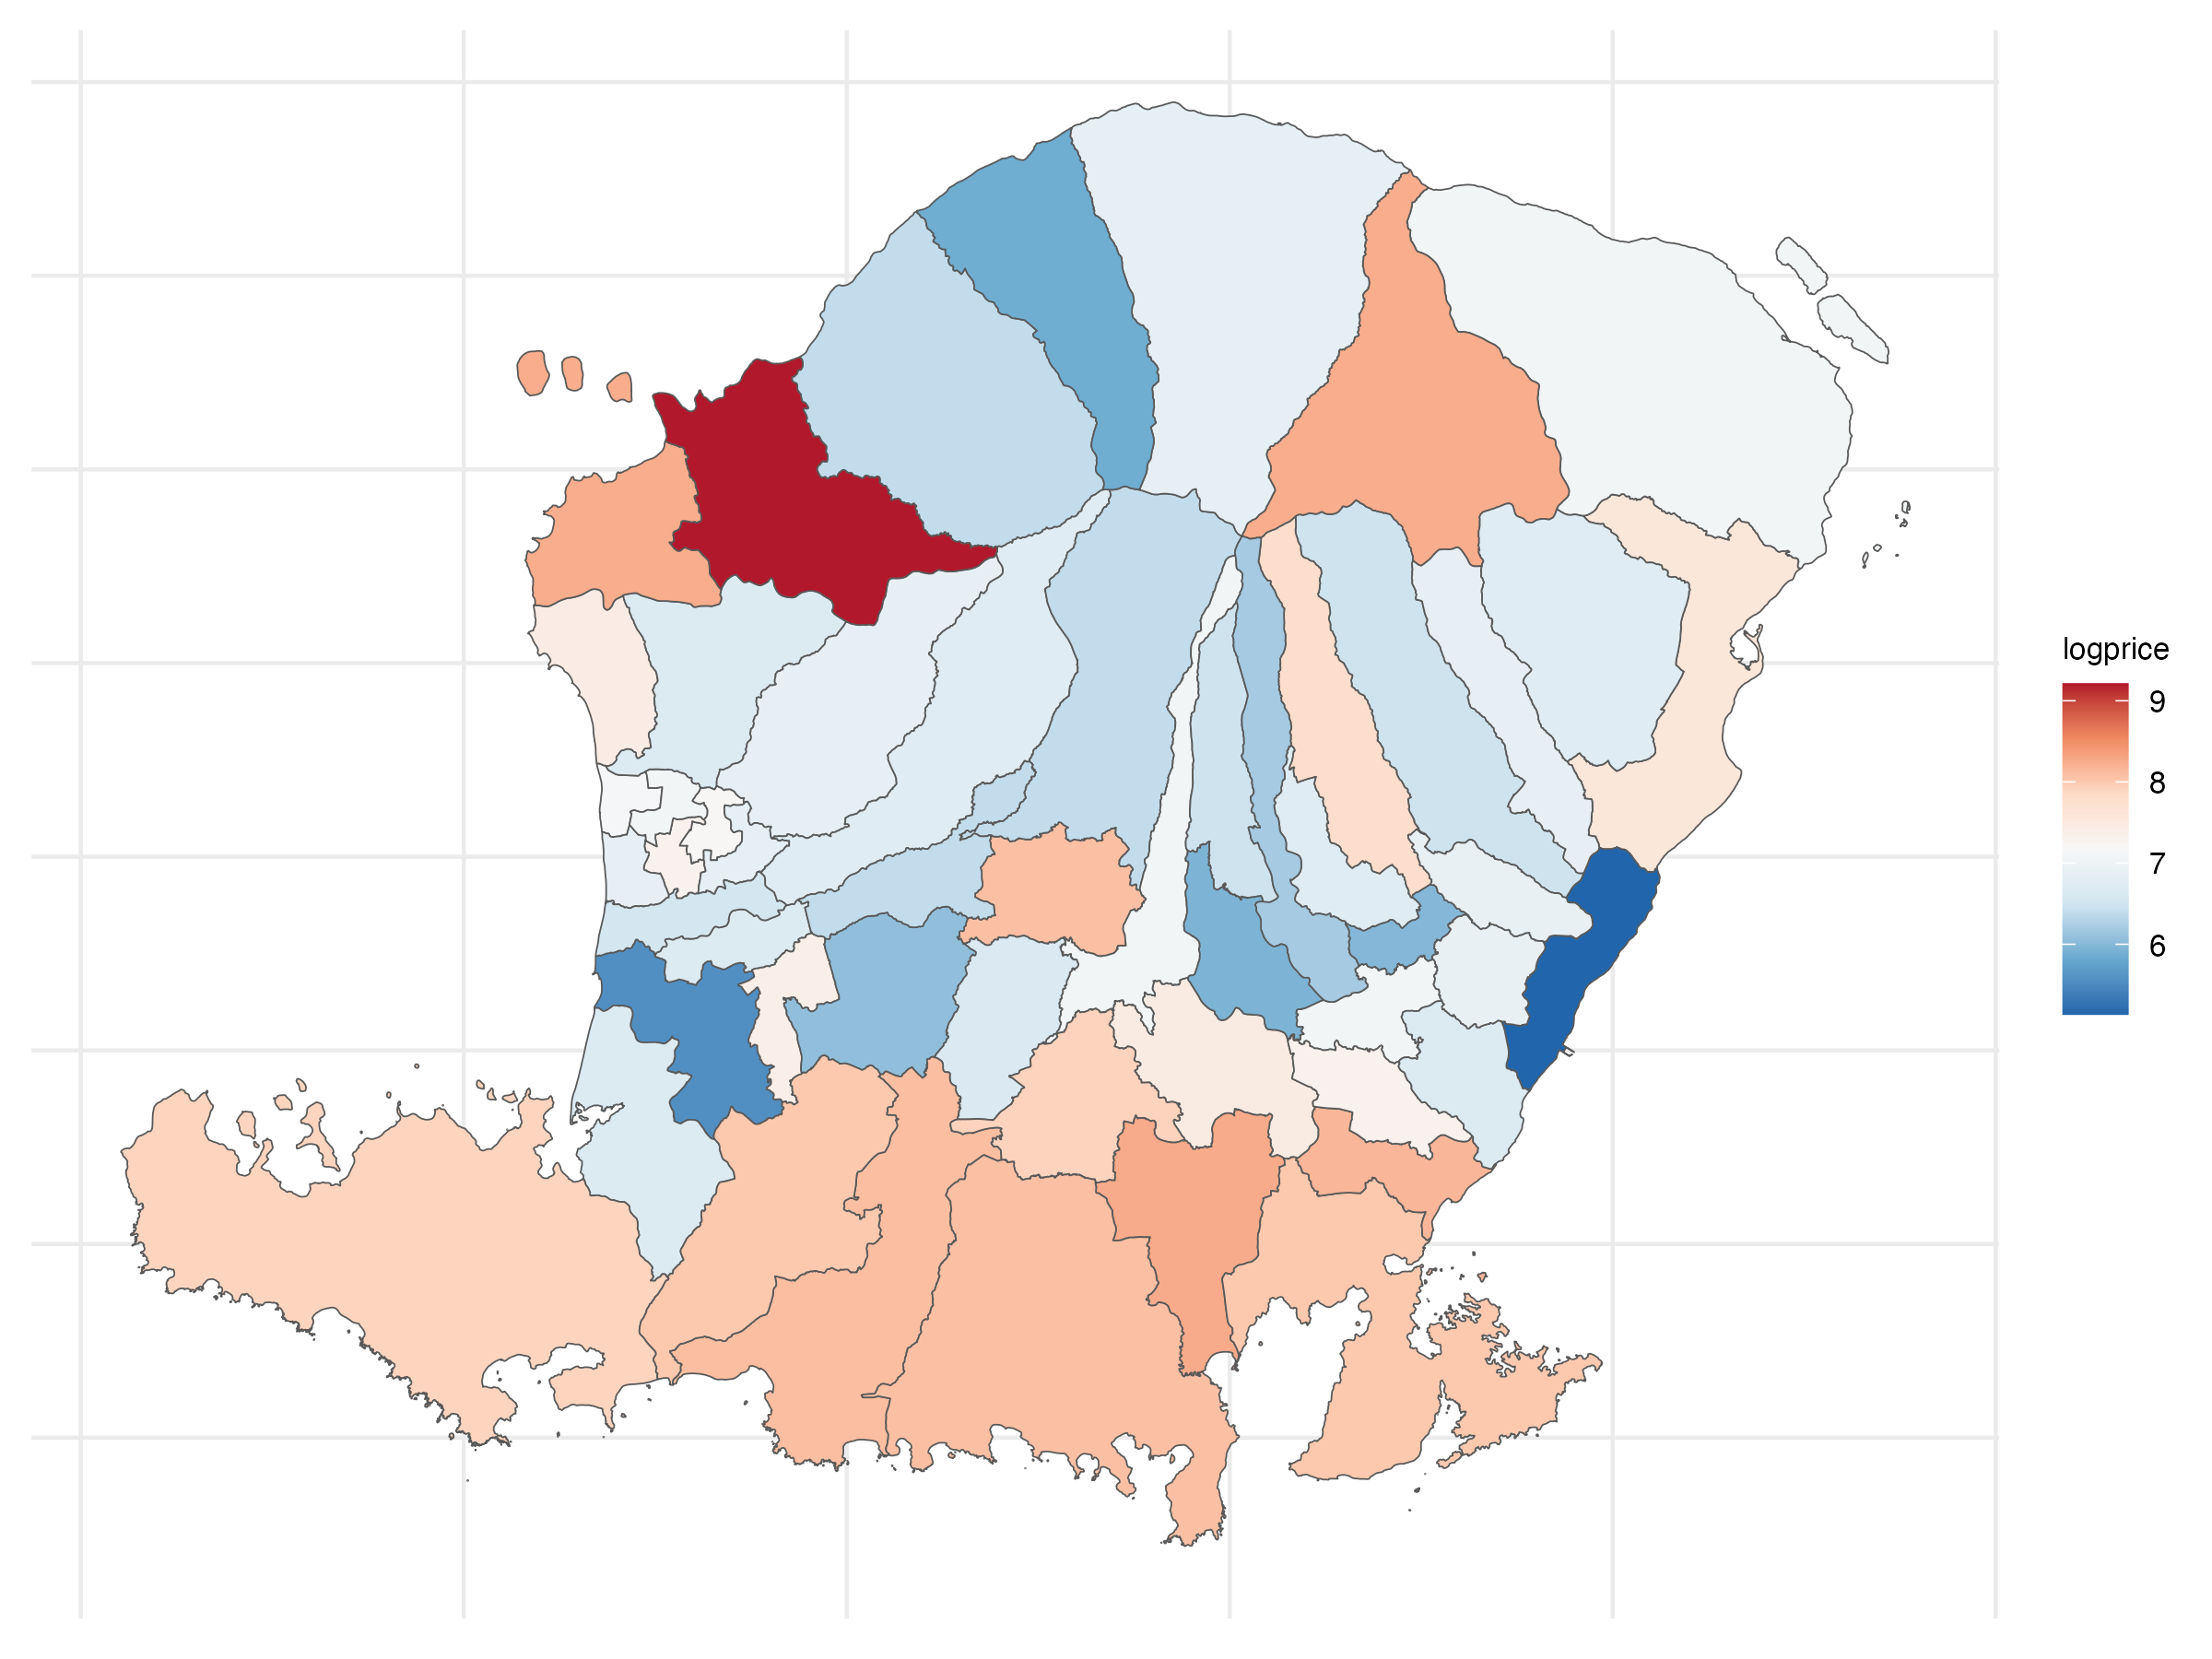
\includegraphics{figures/logprice_map.png}

}

\subcaption{\label{fig-pricenphi2}Aggregate price data (log scale)}

\end{minipage}%

\caption{\label{fig-pricenphi}Heatmap of aggregated price data and phi
values in each Lombok sub-district}

\end{figure}%

\textsubscript{Source:
\href{https://indiraputeri-phd.github.io/CAR_simcomp/manuscript.qmd.html}{Article
Notebook}}

Figure~\ref{fig-pricenphi1} and Figure~\ref{fig-pricenphi2} respectively
present spatial heatmaps illustrating the distribution of estimated
spatial random effects (\(\phi\)) from the CAR model and the average
log-transformed house prices per sub-district accross Lombok island.

Here, the \(\phi\) values represent the spatially structured residuals
not explained by the observed covariates in the CAR model. Specifically,
it captures latent spatial influences such as neighbourhood
desirability, access to infrastructure, or even local policy, that
affect house prices beyond what structural features like land and
building size can account for.

Because the model uses log-transformed prices, \(\phi\) has
multiplicative interpretation on the original price scale. For instance,
if \(\phi = 0.57\) for a given sub-district, then after accounting for
covariates, properties in that area are estimated to be approximately
\(exp(0.57) \approx 1.76\) or 76\% more expensive than average.
Similarly, a sub-district with \(\phi = -0.2\), this suggests that
properties in that area are approximately 18\% less expensive than
average, since \(exp(-0.2) \approx 0.82\).

\section{Results and Discussion}\label{results-and-discussion}

The findings from simulation consistently indicate that both the CAR and
mlvCAR model outperform the other models in capturing spatial
dependencies. This is evidenced by lower RMSE values and reduced bias
across various dataset scenarios, highlighting the CAR model's
robustness. In datasets with strong spatial structures, such as those
generated under \(CAR\) and \(SAR + CAR\) conditions, the CAR model
achieves substantially lower RMSE values compared to GLM and SAR,
suggesting its effectiveness in handling localised spatial variations.

In the context of house price modelling, it is common to encounter
multiple sales observations within a single area, yet precise
coordinates for each sale are often unavailable. Obtaining precise
geographic coordinates in real-world datasets is often challenging due
to limitations in data collection, privacy concerns, or the aggregation
of data into broader administrative units. This limitation renders
point-level approaches, such as GWR, less effective. With multiple
observations available for each area, models like mlvCAR offer a more
practical and accurate solution, effectively capturing spatial
dependencies at an area level without requiring precise point-level
locations.

The results underscore the importance of using models that explicitly
account for spatial dependencies in fields like property valuation,
where spatial heterogeneity plays a significant role. The superior
performance of the CAR model, particularly in datasets with strong
spatial structure, suggests that it may be a more reliable choice for
applications where local spatial variations are critical. The findings
align with previous studies indicating that CAR models are better suited
for managing spatial autocorrelation and heterogeneity, especially when
spatial dependencies are strong.

Spatial maps of the estimated random effects \(\phi\) from the CAR model
offer further insight into the spatial structure of housing prices
across Lombok Island. These effects represent residual spatial patterns
after accounting for structural covariates like land size, building
size, and number of rooms. Such interpretability supports the use of CAR
models not only for improved prediction but also for spatial
diagnostics. The visual comparison of \(\phi\) values and aggregated
log-transformed prices (as shown in Figure~\ref{fig-pricenphi})
highlights spatial patterns that may warrant further
investigation---such as clusters of residual over- or under-prediction
in West and East Lombok respectively. These patterns underscore the
added value of CAR-type models in revealing latent geographic effects.

These findings echo the limitations of GWR when precise coordinates are
lacking, affirming the relevance of area-level approaches. Moreover,
while we use a binary adjacency matrix for consistency, we recognise
that the choice of spatial weight \(\mathbf{W}\) may influences model
performance. Future studies should explore alternative specifications
such as row-standardized or distance-decay matrices to assess their
impact on robustness and interpretability.

Additionally, while the spatial dependence parameter \(\rho\) is
estimated as part of the model fitting, its variability across
simulations suggests that further sensitivity analyses---especially
under different fixed \(\rho\) values---could shed light on model
stability in different spatial contexts.

Additionally, the limitations of point-level models such as GWR in the
absence of precise location data highlight a practical challenge in
spatial modeling. When only area-level data is available, the use of
models like mlvCAR becomes essential, as it allows for spatial analysis
without the need for detailed coordinates, thus expanding the
applicability of spatial models in real-world settings. These insights
suggest potential for further exploration of the CAR and mlvCAR models
in various domains, especially in urban planning, real estate, and other
fields where spatial relationships impact outcomes. Future research
could examine the use of CAR and mlvCAR models with different spatial
resolutions or apply these models to other datasets with varying levels
of spatial dependency to further validate their effectiveness.

In summary, this study highlights the importance of explicitly modeling
spatial dependence in house price analysis. CAR and mlvCAR models emerge
as practical and theoretically sound options, especially when
high-resolution spatial data are unavailable. Future research may extend
these models to finer spatial scales, incorporate additional spatial
diagnostics, or apply them in other domains where spatial heterogeneity
significantly influences outcomes.

\section*{Supplementary information}\label{supplementary-information}
\addcontentsline{toc}{section}{Supplementary information}

Not applicable

\section*{Acknowledgments}\label{acknowledgments}
\addcontentsline{toc}{section}{Acknowledgments}

Not applicable

\section*{Declarations}\label{declarations}
\addcontentsline{toc}{section}{Declarations}

\begin{itemize}
\tightlist
\item
  Funding
\item
  Competing interests
\end{itemize}

No, I declare that the authors have no competing interests as defined by
Springer, or other interests that might be perceived to influence the
results and/or discussion reported in this paper.

\begin{itemize}
\tightlist
\item
  Ethics approval
\item
  Consent to participate
\item
  Consent for publication
\item
  Availability of data and materials
\item
  Code availability
\item
  Authors' contributions
\end{itemize}

\section*{Appendix}\label{appendix}
\addcontentsline{toc}{section}{Appendix}

\subsection*{Bias values for Area-level
Data}\label{bias-values-for-area-level-data}
\addcontentsline{toc}{subsection}{Bias values for Area-level Data}

\begin{table}

\caption{\label{tbl-bias1}Mean ± SD values for bias across different
area-level datasets and parameters. This table presents the mean and
standard deviation (SD) of bias values across area-level datasets (CAR,
SAR + CAR, GWR) and spatial models (GLM, SAR, CAR), with
\(nsim = 1000\). This is also act as numerical representation of fig.~5
(top panel)}

\centering{

\centering\begingroup\fontsize{9}{11}\selectfont

\begin{tabular}[t]{lccc}
\toprule
\multicolumn{1}{c}{ } & \multicolumn{3}{c}{Mean ± SD} \\
\cmidrule(l{3pt}r{3pt}){2-4}
Dataset & GLM & SAR & CAR\\
\midrule
\addlinespace[0.3em]
\multicolumn{4}{l}{\textbf{$\beta_{1}$}}\\
\hspace{1em}CAR & $7.80e-02 \pm 0.1900$ & $9.00e-03 \pm 0.1900$ & $-8.70e-02 \pm 0.1800$\\
\hspace{1em}SAR + CAR & $3.30e-01 \pm 0.3800$ & $2.77e-01 \pm 0.3700$ & $2.10e-01 \pm 0.3500$\\
\hspace{1em}GWR & $-6.00e-02 \pm 0.1100$ & $-6.50e-02 \pm 0.1100$ & $-6.50e-02 \pm 0.1100$\\
\addlinespace[0.3em]
\multicolumn{4}{l}{\textbf{$\beta_{2}$}}\\
\hspace{1em}CAR & $2.19e-01 \pm 0.1500$ & $2.37e-01 \pm 0.1400$ & $2.46e-01 \pm 0.1400$\\
\hspace{1em}SAR + CAR & $-2.47e-01 \pm 0.3900$ & $-2.29e-01 \pm 0.3600$ & $-2.12e-01 \pm 0.3700$\\
\hspace{1em}GWR & $3.05e-01 \pm 0.0900$ & $3.02e-01 \pm 0.0900$ & $3.04e-01 \pm 0.0900$\\
\addlinespace[0.3em]
\multicolumn{4}{l}{\textbf{$\beta_{3}$}}\\
\hspace{1em}CAR & $-1.24e-01 \pm 0.2000$ & $0.00e+00 \pm 0.1900$ & $-3.80e-02 \pm 0.1800$\\
\hspace{1em}SAR + CAR & $-5.80e-02 \pm 0.3700$ & $6.30e-02 \pm 0.3500$ & $-5.00e-03 \pm 0.3500$\\
\hspace{1em}GWR & $-6.20e-02 \pm 0.1100$ & $-3.50e-02 \pm 0.1100$ & $-5.90e-02 \pm 0.1100$\\
\addlinespace[0.3em]
\multicolumn{4}{l}{\textbf{$\beta_{4}$}}\\
\hspace{1em}CAR & $1.83e-01 \pm 0.1600$ & $1.27e-01 \pm 0.1500$ & $1.64e-01 \pm 0.1500$\\
\hspace{1em}SAR + CAR & $1.22e-01 \pm 0.3000$ & $7.60e-02 \pm 0.2900$ & $1.10e-01 \pm 0.2800$\\
\hspace{1em}GWR & $1.82e-01 \pm 0.0900$ & $1.73e-01 \pm 0.0900$ & $1.83e-01 \pm 0.0900$\\
\bottomrule
\end{tabular}
\endgroup{}

}

\end{table}%

\textsubscript{Source:
\href{https://indiraputeri-phd.github.io/CAR_simcomp/manuscript.qmd.html}{Article
Notebook}}

\begin{table}

\caption{\label{tbl-bias2}Mean ± SD values for bias across different
point-level datasets and parameters. This table presents the mean and
standard deviation (SD) of bias values across point-level datasets (CAR,
SAR + CAR, GWR) and spatial models (GLM, SAR, CAR), with
\(nsim = 1000\). This is also act as numerical representation of fig.~5
(bottom panel)}

\centering{

\centering\begingroup\fontsize{9}{11}\selectfont

\begin{tabular}[t]{lccc}
\toprule
\multicolumn{1}{c}{ } & \multicolumn{3}{c}{Mean ± SD} \\
\cmidrule(l{3pt}r{3pt}){2-4}
Dataset & GLMM & GWR & mlvCAR\\
\midrule
\addlinespace[0.3em]
\multicolumn{4}{l}{\textbf{$\beta_{1}$}}\\
\hspace{1em}CAR & $2.80e-04 \pm 0.0115$ & $8.77e-03 \pm 0.0160$ & $-2.00e-05 \pm 0.0114$\\
\hspace{1em}SAR + CAR & $4.06e-03 \pm 0.0525$ & $9.00e-03 \pm 0.0538$ & $9.80e-04 \pm 0.0524$\\
\hspace{1em}GWR & $-5.00e-04 \pm 0.0109$ & $-5.20e-04 \pm 0.0108$ & $-5.40e-04 \pm 0.0108$\\
\addlinespace[0.3em]
\multicolumn{4}{l}{\textbf{$\beta_{2}$}}\\
\hspace{1em}CAR & $-3.10e-04 \pm 0.0125$ & $-5.50e-03 \pm 0.0172$ & $-1.70e-04 \pm 0.0124$\\
\hspace{1em}SAR + CAR & $-2.81e-03 \pm 0.0588$ & $-5.72e-03 \pm 0.0602$ & $-1.02e-03 \pm 0.0585$\\
\hspace{1em}GWR & $9.54e-03 \pm 0.0113$ & $9.55e-03 \pm 0.0113$ & $9.56e-03 \pm 0.0113$\\
\addlinespace[0.3em]
\multicolumn{4}{l}{\textbf{$\beta_{3}$}}\\
\hspace{1em}CAR & $3.80e-04 \pm 0.0096$ & $-2.86e-03 \pm 0.0142$ & $4.50e-04 \pm 0.0095$\\
\hspace{1em}SAR + CAR & $9.00e-04 \pm 0.0391$ & $-8.00e-04 \pm 0.0405$ & $1.67e-03 \pm 0.0389$\\
\hspace{1em}GWR & $-4.90e-04 \pm 0.0092$ & $-5.00e-04 \pm 0.0091$ & $-5.20e-04 \pm 0.0091$\\
\addlinespace[0.3em]
\multicolumn{4}{l}{\textbf{$\beta_{4}$}}\\
\hspace{1em}CAR & $-4.30e-04 \pm 0.0089$ & $1.18e-03 \pm 0.0122$ & $-5.10e-04 \pm 0.0089$\\
\hspace{1em}SAR + CAR & $3.10e-04 \pm 0.0393$ & $1.03e-03 \pm 0.0394$ & $-8.00e-05 \pm 0.0391$\\
\hspace{1em}GWR & $1.09e-03 \pm 0.0089$ & $1.05e-03 \pm 0.0088$ & $1.07e-03 \pm 0.0087$\\
\bottomrule
\end{tabular}
\endgroup{}

}

\end{table}%

\textsubscript{Source:
\href{https://indiraputeri-phd.github.io/CAR_simcomp/manuscript.qmd.html}{Article
Notebook}}

\subsection*{Model Comparison for area-level
data}\label{model-comparison-for-area-level-data}
\addcontentsline{toc}{subsection}{Model Comparison for area-level data}

\begin{table}

\caption{\label{tbl-modelcomp1}This table compares the performance of
GLM, SAR, and CAR models on area-level data. It reports parameter
estimates (with 95\% confidence intervals), spatial parameters
(\(\rho\)), variances (\(\nu^2\), \(\tau^2\)), and model fit criteria
(AIC, DIC, WAIC, LMPL, log-likelihood). The results highlight each
model's capability to capture spatial dependencies and variability}

\centering{

\centering\begingroup\fontsize{9}{11}\selectfont

\begin{tabular}[t]{llll}
\toprule
 & GLM & SAR & CAR\\
\midrule
\addlinespace[0.3em]
\multicolumn{4}{l}{\textbf{Coefficients}}\\
\hspace{1em}Intercept & 7.19 [7.02, 7.35]* & 6.92 [6.48, 7.37]* & 7.19 [7.03, 7.35]*\\
\hspace{1em}Land-size & 0.45 [0.24, 0.66]* & 0.45 [0.25, 0.64]* & 0.45 [0.23, 0.65]*\\
\hspace{1em}Built-up area & 0.01 [-0.20, 0.23] & 0.01 [-0.18, 0.22] & 0.02 [-0.20, 0.23]\\
\hspace{1em}No. of bedroom & -0.20 [-0.43, 0.02] & -0.23 [-0.45, -0.01]* & -0.21 [-0.44, 0.02]\\
\hspace{1em}No. of bathroom & 0.54 [0.33, 0.76]* & 0.56 [0.36, 0.77]* & 0.55 [0.34, 0.76]*\\
\addlinespace[0.3em]
\multicolumn{4}{l}{\textbf{Spatial parameter}}\\
\hspace{1em}$\rho$ & - & 0.009[-0.005, 0.023] & 0.39 [0.01, 0.91]*\\
\addlinespace[0.3em]
\multicolumn{4}{l}{\textbf{Variances}}\\
\hspace{1em}$\nu^2$ & 0.31 [0.21, 0.45]* & 0.27 [0.19, 0.41]* & 0.28 [0.01, 0.44]*\\
\hspace{1em}$\tau^2$ & 0.20 [0.11, 0.34]* & - & 0.04 [0.01, 0.91]*\\
\addlinespace[0.3em]
\multicolumn{4}{l}{\textbf{Model fit criterion}}\\
\hspace{1em}AIC & - & - & -\\
\hspace{1em}DIC & 94.73 & 94.73 & 82.52\\
\hspace{1em}WAIC & 95.64 & - & 87.43\\
\hspace{1em}LMPL & -48.04 & - & -46.71\\
\hspace{1em}Log-likelihood & -41.49 & -41.36 & -37.29\\
\bottomrule
\end{tabular}
\endgroup{}

}

\end{table}%

\textsubscript{Source:
\href{https://indiraputeri-phd.github.io/CAR_simcomp/manuscript.qmd.html}{Article
Notebook}}

\subsection*{Example of beta-values in GWR
model}\label{example-of-beta-values-in-gwr-model}
\addcontentsline{toc}{subsection}{Example of beta-values in GWR model}

\phantomsection\label{cell-fig-betaplot}
\begin{figure}[H]

\centering{

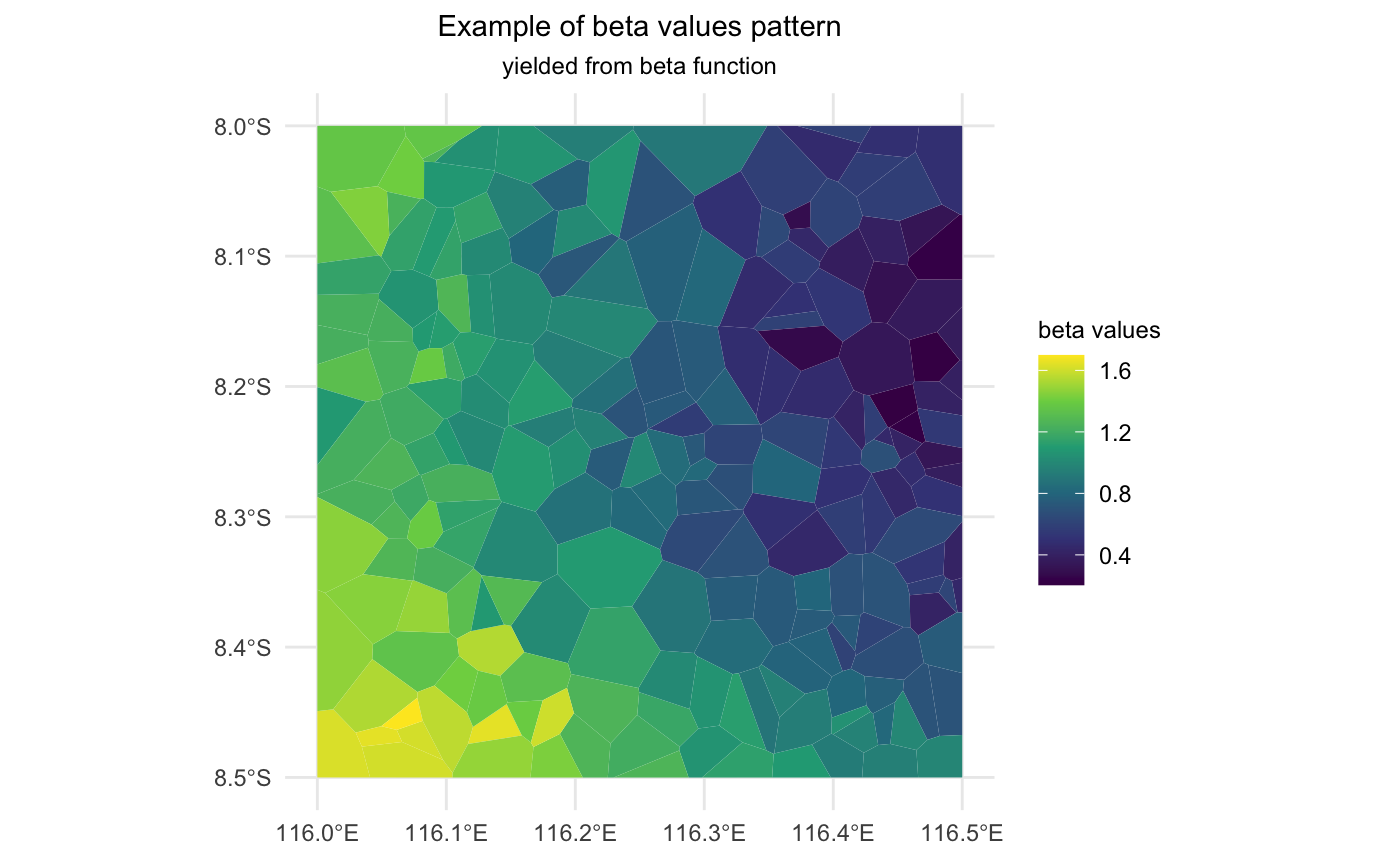
\includegraphics[width=0.9\textwidth,height=\textheight]{figures/betavalues_plot.png}

}

\caption{\label{fig-betaplot}Spatial variation of \(\beta\) values
generated using a custom beta function. The color gradient represents
the magnitude of \(\beta\) values across the artificial study region,
highlighting localised patterns and heterogeneity. The visualisation
demonstrates the spatially varying coefficient structure modeled in the
study}

\end{figure}%

\textsubscript{Source:
\href{https://indiraputeri-phd.github.io/CAR_simcomp/manuscript.qmd.html}{Article
Notebook}}

\section*{References}\label{references}
\addcontentsline{toc}{section}{References}

\phantomsection\label{refs}
\begin{CSLReferences}{1}{0}
\bibitem[\citeproctext]{ref-anselin2013spatial}
Anselin, Luc. 2013. \emph{Spatial Econometrics: Methods and Models}.
Vol. 4. Springer Science \& Business Media.

\bibitem[\citeproctext]{ref-anselin1988spatial}
Anselin, Luc, and Daniel A Griffith. 1988. {``Do Spatial Effecfs Really
Matter in Regression Analysis?''} \emph{Papers in Regional Science} 65
(1): 11--34.

\bibitem[\citeproctext]{ref-banerjee2014hierarchical}
Banerjee, Sudipto, Bradley P Carlin, and Alan E Gelfand. 2014.
\emph{Hierarchical Modeling and Analysis for Spatial Data}. CRC press.

\bibitem[\citeproctext]{ref-begueria2009comparison}
Beguería, Santiago, and Yolanda Pueyo. 2009. {``A Comparison of
Simultaneous Autoregressive and Generalized Least Squares Models for
Dealing with Spatial Autocorrelation.''} \emph{Global Ecology and
Biogeography} 18 (3): 273--79.

\bibitem[\citeproctext]{ref-besag1991bayesian}
Besag, Julian, Jeremy York, and Annie Mollié. 1991. {``Bayesian Image
Restoration, with Two Applications in Spatial Statistics.''}
\emph{Annals of the Institute of Statistical Mathematics} 43 (March):
1--20. \url{https://doi.org/10.1007/BF00116466}.

\bibitem[\citeproctext]{ref-bottero2017buildings}
Bottero, Marta, Marina Bravi, Giulio Mondini, and Antonio Talarico.
2017. {``Buildings Energy Performance and Real Estate Market Value: An
Application of the Spatial Auto Regressive (SAR) Model.''}
\emph{Appraisal: From Theory to Practice: Results of SIEV 2015},
221--30.

\bibitem[\citeproctext]{ref-brunsdon1996geographically}
Brunsdon, Chris, A Stewart Fotheringham, and Martin E Charlton. 1996.
{``Geographically Weighted Regression: A Method for Exploring Spatial
Nonstationarity.''} \emph{Geographical Analysis} 28 (4): 281--98.

\bibitem[\citeproctext]{ref-cellmer2020spatial}
Cellmer, Radosław, Aneta Cichulska, and Mirosław Bełej. 2020. {``Spatial
Analysis of Housing Prices and Market Activity with the Geographically
Weighted Regression.''} \emph{ISPRS International Journal of
Geo-Information} 9 (6): 380. \url{https://doi.org/10.3390/ijgi9060380}.

\bibitem[\citeproctext]{ref-cellmer2019application}
Cellmer, Radosław, Katarzyna Kobylińska, and Mirosław Bełej. 2019.
{``Application of Hierarchical Spatial Autoregressive Models to Develop
Land Value Maps in Urbanized Areas.''} \emph{ISPRS International Journal
of Geo-Information} 8 (4): 195.

\bibitem[\citeproctext]{ref-de2012bayesian}
De Oliveira, Victor. 2012. {``Bayesian Analysis of Conditional
Autoregressive Models.''} \emph{Annals of the Institute of Statistical
Mathematics} 64: 107--33.

\bibitem[\citeproctext]{ref-droj2024comprehensive}
Droj, Gabriela, Anita Kwartnik-Pruc, and Laurențiu Droj. 2024. {``A
Comprehensive Overview Regarding the Impact of GIS on Property
Valuation.''} \emph{ISPRS International Journal of Geo-Information} 13
(6): 175.

\bibitem[\citeproctext]{ref-elhorst2014spatial}
Elhorst, J Paul et al. 2014. \emph{Spatial Econometrics: From
Cross-Sectional Data to Spatial Panels}. Vol. 479. Springer.

\bibitem[\citeproctext]{ref-elhorst2012model}
Elhorst, J Paul, Donald J Lacombe, and Gianfranco Piras. 2012. {``On
Model Specification and Parameter Space Definitions in Higher Order
Spatial Econometric Models.''} \emph{Regional Science and Urban
Economics} 42 (1-2): 211--20.

\bibitem[\citeproctext]{ref-fix2021simultaneous}
Fix, Miranda J, Daniel S Cooley, and Emeric Thibaud. 2021.
{``Simultaneous Autoregressive Models for Spatial Extremes.''}
\emph{Environmetrics} 32 (2): e2656.

\bibitem[\citeproctext]{ref-golgher2016interpret}
Golgher, André Braz, and Paul R Voss. 2016. {``How to Interpret the
Coefficients of Spatial Models: Spillovers, Direct and Indirect
Effects.''} \emph{Spatial Demography} 4: 175--205.

\bibitem[\citeproctext]{ref-lee2013carbayes}
Lee, Duncan. 2013. {``CARBayes: An r Package for Bayesian Spatial
Modeling with Conditional Autoregressive Priors.''} \emph{Journal of
Statistical Software} 55 (13): 1--24.
\url{https://doi.org/10.18637/jss.v055.i13}.

\bibitem[\citeproctext]{ref-leroux2000estimation}
Leroux, Brian G, Xingye Lei, and Norman Breslow. 2000. {``Estimation of
Disease Rates in Small Areas: A New Mixed Model for Spatial
Dependence.''} In \emph{Statistical Models in Epidemiology, the
Environment, and Clinical Trials}, 179--91.

\bibitem[\citeproctext]{ref-LeSage2014}
LeSage, James P., and R. Kelley Pace. 2014. {``Interpreting Spatial
Econometric Models.''} In \emph{Handbook of Regional Science}, edited by
Manfred M. Fischer and Peter Nijkamp, 1535--52. Berlin, Heidelberg:
Springer Berlin Heidelberg.
\url{https://doi.org/10.1007/978-3-642-23430-9_91}.

\bibitem[\citeproctext]{ref-lu2011geographically}
Lu, Binbin, Martin Charlton, and A Stewart Fotheringham. 2011.
{``Geographically Weighted Regression Using a Non-Euclidean Distance
Metric with a Study on London House Price Data.''} \emph{Procedia
Environmental Sciences} 7: 92--97.

\bibitem[\citeproctext]{ref-mccord2014understanding}
McCord, Michael, Peadar T Davis, Martin Haran, David McIlhatton, and
John McCord. 2014. {``Understanding Rental Prices in the UK: A
Comparative Application of Spatial Modelling Approaches.''}
\emph{International Journal of Housing Markets and Analysis} 7 (1):
98--128.

\bibitem[\citeproctext]{ref-morris2019bayesian}
Morris, Mitzi, Katherine Wheeler-Martin, Dan Simpson, Stephen J Mooney,
Andrew Gelman, and Charles DiMaggio. 2019. {``Bayesian Hierarchical
Spatial Models: Implementing the Besag York Molli{é} Model in Stan.''}
\emph{Spatial and Spatio-Temporal Epidemiology} 31 (November): 100301.
\url{https://doi.org/10.1016/j.sste.2019.100301}.

\bibitem[\citeproctext]{ref-pagourtzi2003real}
Pagourtzi, Elli, Vassilis Assimakopoulos, Thomas Hatzichristos, and Nick
French. 2003. {``Real Estate Appraisal: A Review of Valuation
Methods.''} \emph{Journal of Property Investment \& Finance} 21 (4):
383--401.

\bibitem[\citeproctext]{ref-rue2005gaussian}
Rue, Havard, and Leonhard Held. 2005. \emph{Gaussian Markov Random
Fields: Theory and Applications}. Chapman; Hall/CRC.

\bibitem[\citeproctext]{ref-sarlas2015localized}
Sarlas, Georgios, and Kay W Axhausen. 2015. {``Localized Speed
Prediction with the Use of Spatial Simultaneous Autoregressive
Models.''} In \emph{TRB 94th Annual Meeting Compendium of Papers}.
National Academy of Sciences.

\bibitem[\citeproctext]{ref-sisman2022modelling}
Sisman, Suleyman, and Arif Cagdas Aydinoglu. 2022. {``A Modelling
Approach with Geographically Weighted Regression Methods for Determining
Geographic Variation and Influencing Factors in Housing Price: A Case in
Istanbul.''} \emph{Land Use Policy} 119 (August): 106183.
\url{https://doi.org/10.1016/j.landusepol.2022.106183}.

\bibitem[\citeproctext]{ref-soltani2021housing}
Soltani, Ali, Christopher James Pettit, Mohammad Heydari, and Fatemeh
Aghaei. 2021. {``Housing Price Variations Using Spatio-Temporal Data
Mining Techniques.''} \emph{Journal of Housing and the Built
Environment} 36 (3): 1--29.
\url{https://doi.org/10.1007/s10901-020-09811-y}.

\bibitem[\citeproctext]{ref-stern1999inference}
Stern, Hal, and Noel A Cressie. 1999. {``Inference for Extremes in
Disease Mapping.''} \emph{John Wiley and Sons} 11: 63--84.

\bibitem[\citeproctext]{ref-stewart2018localized}
Stewart Fotheringham, A, and Bumsub Park. 2018. {``Localized
Spatiotemporal Effects in the Determinants of Property Prices: A Case
Study of Seoul.''} \emph{Applied Spatial Analysis and Policy} 11
(August): 581--98. \url{https://doi.org/10.1007/s12061-017-9232-8}.

\bibitem[\citeproctext]{ref-trojanek2018spatial}
Trojanek, Radoslaw, and Michal Gluszak. 2018. {``Spatial and Time Effect
of Subway on Property Prices.''} \emph{Journal of Housing and the Built
Environment} 33 (October): 359--84.
\url{https://doi.org/10.1007/s10901-017-9569-y}.

\bibitem[\citeproctext]{ref-van2011mice}
Van Buuren, Stef, and Karin Groothuis-Oudshoorn. 2011. {``Mice:
Multivariate Imputation by Chained Equations in r.''} \emph{Journal of
Statistical Software} 45: 1--67.

\bibitem[\citeproctext]{ref-ver2018spatial}
Ver Hoef, Jay M, Erin E Peterson, Mevin B Hooten, Ephraim M Hanks, and
Marie-Josèe Fortin. 2018. {``Spatial Autoregressive Models for
Statistical Inference from Ecological Data.''} \emph{Ecological
Monographs} 88 (1): 36--59.

\bibitem[\citeproctext]{ref-wall2004close}
Wall, Melanie M. 2004. {``A Close Look at the Spatial Structure Implied
by the CAR and SAR Models.''} \emph{Journal of Statistical Planning and
Inference} 121 (2): 311--24.

\bibitem[\citeproctext]{ref-wang2020geographically}
Wang, Chih-Hao, and Na Chen. 2020. {``A Geographically Weighted
Regression Approach to Investigating Local Built-Environment Effects on
Home Prices in the Housing Downturn, Recovery, and Subsequent
Increases.''} \emph{Journal of Housing and the Built Environment} 35:
1283--1302.

\bibitem[\citeproctext]{ref-yang2019does}
Yang, Linchuan, Jiangping Zhou, Oliver F Shyr, et al. 2019. {``Does Bus
Accessibility Affect Property Prices?''} \emph{Cities} 84 (January):
56--65. \url{https://doi.org/10.1016/j.cities.2018.07.005}.

\bibitem[\citeproctext]{ref-yu2007modeling}
Yu, Danlin. 2007. {``Modeling Owner-Occupied Single-Family House Values
in the City of Milwaukee: A Geographically Weighted Regression
Approach.''} \emph{GIScience \& Remote Sensing} 44 (3): 267--82.

\end{CSLReferences}



\end{document}
